\chapter{基于邻域结构迁移的多目标旅行商问题求解算法}
\label{chap:NST}

\section{引言}
\label{sec:NST:引言}
很多现实中的问题都是由相互冲突和影响的多个目标组成,并且在给定条件下,问题的多个目标需要同时达到最佳,这类问题被称作MOP。当问题的变量域为有限集合时,这类问题就可以被称为CMOP。MOTSP是具有多个冲突的目标的CMOP,并且在大部分行业都可见,包括但不限于交通运输、网络通信和钻孔电路板等领域。由于其变量域所演变出的组合数巨大(NP难),传统的确定性算法难以在一定时间内给出这类问题的解决方案。因此,设计能够在合理时间内给出近似解决方案的启发式方法,就成了求解这类问题的关键。
\par
自多目标组合优化被提出后,研究者们就针对CMOP设计了一系列的MOEA,其大多数是基于EA,可主要分为三大类:基于Pareto支配关系的MOEA\cite{zitzler1999multiobjective,deb2002fast,knowles2000approximating,yang2013grid,laumanns2002combining,hadka2013borg,le2009improved,aguirre2010hybrid,aguirre2013adaptive}、基于指标的MOEA\cite{zitzler2004indicator,bringmann2011approximation,brockhoff20152,rudolph2013evenly,beume2007sms,wagner2007pareto}和基于分解的MOEA\cite{zhang2007moea,zhang2009performance,li2014evolutionary,cheng2016reference,cai2016decomposition,yuan2015balancing}。但是,在应对某些高维度的CMOP,基于Pareto支配关系和基于指标的MOEA都有着其本身的缺陷处。因为在高维度解集中,包含的几乎都是非支配的解,这就导致了只用Pareto支配关系无法区分这些非支配解的优劣,从而不能够均匀且广泛的选出下一代进化的种群。同样,基于指标的MOEA因其指标算法的高复杂度,使得它们在高维度问题中会耗费大量计算资源。然而,基于分解的MOEA因其分解的策略,使得它们被广泛的应用于CMOP中,这使得这种基于分解的方法在过去的十几年中,成为了处理CMOP的最突出的方法之一。一个代表性的算法是MOEA/D\cite{zhang2007moea},其核心思想就是把一个CMOP通过权重向量分解成一组单目标子问题,然后根据各子问题之间的相似度关系构成邻居关系,然后利用邻居子问题之间的信息对所有子问题进行优化。
\par
近年来,利用机器学习中相关的思想来进一步提高MOEA的效率,成为了当下研究的热点。在进化优化的背景下,基于迁移学习(TL)中利用跨问题领域的有用特征数据来提高学习性能这一方法,已经有很多研究者开始将其应用到CMOP当中,并将其与进化算法相结合,提出了进化迁移优化(ETO)\cite{feng2020explicit,lin2020effective,tan2021evolutionary}。在章节~\ref{sec:背景介绍:进化迁移优化}~中可以了解到,在多目标和超多目标优化中的知识信息可以采用非支配解集等形式来实现跨问题的迁移。当ETO与基于分解的MOEA相结合时,分解得来的一系列子问题之间拥有天然的联系,这使得所属子问题的知识能够很好的被迁移到其他子问题上,通过不同子问题之间的相互促进,以此来提高算法的整体效率和质量。
% \par
% 由此,将基于分解的MOEA和ETO相结合,以此来针对CMOP来进行算法设计,是本章研究的重点。由于在ETO中,所使用的知识信息与所求问题密切相关,且本章将使用邻域结构(章节~\ref{subsec:背景介绍:局部搜索:邻域结构})当做被迁移的知识,为此,本章将使用MOTSP问题(章节~\ref{subsec:背景介绍:测试问题:MOTSP})来对设计的算法进行性能测试。

\section{研究动机}
\label{sec:NST:研究动机}
从前面的章节可以了解到,基于分解的MOEA是通过将CMOP分解成一组单目标优化问题,然后对这些单目标问题进行求解,其目的在于将复杂的问题降维,由复杂的CMOP转变成简单的单目标问题,然后可以用解决单目标问题的方法来求解,最后将这些解组合起来就成为了CMOP的解集。并且,在基于分解的方法中最具代表性的MOEA/D中使用了“邻居”的概念,MOEA/D根据被分解后的子问题之间的联系,从而形成子问题间的邻居关系,然后利用子问题之间的联系,通过用当前子问题中的优质解来替换其他邻居子问题中的差解,以此达到不同子问题间的协作效应。
\par
当求解的问题的目标数少时,被分解成的一组单目标优化问题之间存在着“邻居”关系,此时邻居子问题之间还能够依靠着协作来达到相互促进的效果。但是,当求解的问题的目标数变多时,如果依照低维问题的分解粒度,则通过分解得到的单目标问题数量是成指数增加的,这就导致了分解空间的爆炸,若使用算法对如此多的子问题进行优化,这将耗费大量计算资源。如果加大分解的粒度来使得分解得到的子问题恒定,那么这些子问题之间的“邻居”关系将会变得极其微弱,就算当前子问题产生了优质解也难以替换其他子问题的解,这就导致算法的协作效应难以发挥作用。
\par
在进化优化的背景下,ETO利用跨问题领域的知识迁移这一特征能够很好地适用于基于分解的MOEA。因此,可以将ETO的思想融入到基于分解的MOEA当中,在分解得到的子问题之间建立知识迁移模型。因此,使用ETO的目的在于挖掘子问题的内在信息,然后通过迁移的方式将这些信息在不同子问题之间传递使用。然而,通过章节~\ref{sec:背景介绍:进化迁移优化}~可知,现在将ETO应用到CMOP中,大多数是通过将非支配解当做被迁移的信息。然而,通过解迁移的方式,类似于MOEA/D中的协作,如果子问题之间的相似度较低,那么从这些非支配解中能够学习到的有用信息就会很少(解中蕴含的信息本身就少),这些信息很大可能对其他子问题无效,以致产生负迁移,使得难以对问题的优化起到促进作用。
\par
从章节~\ref{subsec:背景介绍:局部搜索:邻域结构}~可以知道,MOTSP可以用邻域结构的方式具现化,这些邻域结构本身就携带了这个问题的大部分特征,并且,邻域结构还能够作为局部搜索算子的一部分。若使用邻域结构来承载子问题的内在信息,容易知道,邻域结构能够承载的信息量要比使用非支配解所蕴含的信息量更多。因此,当以邻域结构作为知识迁移的基本单位,那么就算子问题的相关性变弱,算法也能够从邻域结构中挖掘出一种结构模式,然后使用特定的局部搜索方法来使用该结构,从而促进子问题的优化。
\par
因此,综合章节~\ref{sec:NS_Method:邻域结构生成算法}~提出的邻域结构生成方法,结合基于分解的MOEA和ETO,本章提出了一种基于邻域结构迁移的多目标旅行商问题求解算法(NST-MOEA)。

\section{邻域结构迁移}
\label{sec:NST:邻域结构迁移}
进化迁移优化(ETO)是利用跨问题领域的知识来提高其优化能力的一种方法。容易知道,知识的表达形式,及其如何跨问题迁移是设计算法时的关键点。在提出的邻域结构迁移这一模型中,本章将问题的邻域结构具象化,将邻域结构作为知识迁移的基础单位,视分解得到的多个子问题为不同的问题领域,并且提出了一种由知识关联到问题的两目标相似度模型,该模型能够为每个子问题构造一个知识库,然后使用多臂老虎机模型来获取知识库中的知识,以此达到知识在不同子问题间迁移。

\subsection{子问题}
\label{subsec:NST:邻域结构迁移:子问题}
将CMOP分解成多个子问题的方法有很多,如同章节~\ref{subsec:背景介绍:多目标组合优化算法:基于分解的多目标进化算法}~中介绍的加权和法、切比雪夫法和基于惩罚的边界交叉法。这些分解方法的实质其实是通过聚合的方式,使得CMOP的解的多个维度聚合成一个维度,从而转变为单目标问题。在本章中将提供另外一个分解思路,在对CMOP优化前,就通过权重将该问题分解成不同的子问题,在对问题优化时,每个子问题的解都是单维度的,如若需要可以通过权重将子问题单维度的解还原成多维度的解。
\par
以MOTSP(章节~\ref{subsec:背景介绍:测试问题:MOTSP})为例,给定一组权重向量$\lambda$,有:
\begin{align}
    \label{eq:NST:权重向量}
    & \lambda = \{ \lambda^1, \cdots, \lambda^N \}, \\
    s.t. \quad & \lambda^{i} = [ \lambda^{i}_1, \cdots, \lambda^{i}_m ]^T, \notag \\
    & \forall \lambda^{i}_j \geq 0, \ \sum_{j=1}^m \lambda^{i}_j = 1. \notag
\end{align}
其中,$N$为子问题数,$m$为多目标问题的目标个数,$\lambda^{i}$代表第$i$个子问题的权重向量。假设有一个$m$目标的MOTSP问题$G = (V, E, W)$,其中$V = \{v_1, \cdots, v_n\}$为具有$n$个元素的点集,$E = \{ e_{i,j} = (v_i, v_j) \ | \ v_i, v_j \in V, i \not = j \}$为具有$n(n-1)$个元素的边集,$W$为问题的$m$个边权集,则有:
\begin{align}
    \label{eq:NST:边权矩阵}
    & W = \{ W^1, \cdots, W^m \}, \\
    s.t. \quad & W^k = \{ w^k_{i,j} \ | \ e_{i,j} \in E, i \not = j \}. \notag
\end{align}
其中$W^k$代表第$k$个目标的边权集,$w^k_{i,j}$为边$e_{i,j}$在第$k$个目标上的边权值。则由权重$\mu$对MOTSP问题进行分解,可以得到$N$个子问题$\mathcal{G}$,以$\mathcal{W}$代表这些子问题的边权集,则第$i$个子问题的边权集$\mathcal{W}^i$可以表示为:
\begin{align}
    \label{eq:NST:SP}
    \mathcal{W}^i = \sum_{k=1}^m  \lambda^{i}_k W^i.
\end{align}
容易知道,这些子问题都是单目标的TSP问题,第$i$个子问题可以表示为$\mathcal{G}^i = (V, E, \mathcal{W}^i)$。

\subsection{邻域结构}
\label{subsec:NST:邻域结构迁移:邻域结构}
由章节~\ref{subsec:背景介绍:局部搜索:邻域结构}~可以知道,邻域结构是建立在具体问题的基础之上的。对于TSP问题而言,其邻域结构就是每个顶点只与少数几个顶点相连的稀疏图,该稀疏图也可称为候选集。经由上一节对子问题的介绍可知,当MOTSP问题通过权重向量分解成一组子问题的时,这些子问题其实就是单目标的TSP问题。在本章节中,邻域结构不仅是作为局部搜索的核心结构,同时也是知识迁移的基本单位。所以,在算法中需要在邻域结构和子问题之间建立其映射关系,并将邻域结构也形式化。所以,本节将子问题$\mathcal{G}^k= (V, E, \mathcal{W}^k)$的邻域结构的数学形式表述如下:
\begin{align}
    \label{eq:NST:邻域结构}
    \mathcal{N}^{k} & = \{ \mathcal{N}^{k}_{v_1}, \cdots, \mathcal{N}^{k}_{v_n} \},  \\
    s.t. \quad \mathcal{N}^{k}_{v_i} & = \{ v_1, \cdots, v_j \}, \notag \\
    e_{i,j} & = (v_i,v_j) \in E, \ v_i,v_j \in V, \notag \\
    % & \{ e_{i,1} = (e_i,v_1), \cdots, e_{i,j} = (e_i,v_j) \} \subseteq E, \notag \\
    i,j & \in \{1, \cdots, n\}. \notag
\end{align}
其中,$\mathcal{N}^{k}$为第$k$个子问题的邻域结构,$\mathcal{N}^{k}_{v_i} = \{ v_1, \cdots, v_j \}$为第$k$个子问题中顶点$v_i$的邻域集合,集合中包含$j$个候选点,易知$2 \leq j \leq M$,即邻域集合最少包含$2$个候选点,最多包含$M$个候选点,$M$为邻域修剪时最多能保留的边数。
\par
在章节~\ref{sec:NS_Method:邻域结构生成算法}~中提出了meNS生成方法。在本章中,将使用meNS生成方法为所有子问题生成对应的邻域结构,且以每个点最多保留$M=5$条边的稀疏度来对生成的邻域结构进行修剪。所以,子问题$\mathcal{G}^k = (V, E, \mathcal{W}^k)$的邻域结构为:
\begin{align}
    \label{eq:NST:meNS}
    \mathcal{N}^{k} \xleftarrow[M]{meNS} \mathcal{W}^k.
\end{align}

\subsection{两目标相似度模型}
\label{subsec:NST:邻域结构迁移:两目标相似度模型}
进化迁移优化(ETO)作为近年来较为新颖的方法,在多目标优化领域中,常与其他优化算法相结合的形式在多任务优化当中出现\cite{feng2020explicit,lin2020effective,gupta2016multiobjective}。并且,ETO在多任务优化中具有几个特征:
\begin{itemize}
    \item 任务与任务之间存在相关性,即任务之间具有一定的相似度。
    \item 有知识信息通过任务之间的关联在不同任务之间迁移。
\end{itemize}
其目的在于,使得信息能够在多任务之间进行正迁移,以致于这些信息能够给其它相异的任务起到促进的作用。同理,这些特征在多目标组合优化之中同样适用,当一个多目标组合优化问题分解为多个不同的子问题时,这些子问题之间自然地具有内在的相似性,并且用meNS生成算法为这些子问题生成各自的邻域结构,以这些邻域结构当作信息的载体,然后通过子问题之间的关联来进行邻域结构的迁移,以此达到子问题之间的相互促进。
\par
为了建立子问题和邻域结构之间的映射关系、定量的表示子问题之间的相关性以及邻域结构中所蕴含信息量的多少,下面将介绍两目标相似度模型中关联子问题和邻域结构的两个目标的相关定义。
\par
\begin{definition}
    \label{def:Similarity}
    假设有问题$G = (V,E,W)$,分解向量集$\lambda = \{ \lambda^1, \cdots, \lambda^N \}$,则可得子问题集$\mathcal{G} = \{ \mathcal{G}^1, \cdots , \mathcal{G}^N \}$,如果有子问题$\mathcal{G}^j$和参考子问题$\mathcal{G}^i$,则子问题$\mathcal{G}^j$和参考子问题$\mathcal{G}^i$之间的相似度为两子问题对应的分解权重向量$\lambda^i$与$\lambda^j$之差的$L_2$范数,其数学形式如下:
    \begin{align}
        \label{eq:Similarity}
        & S^i_j  = \|\lambda^j - \lambda^i\|_2, \\
        s.t. \quad & \lambda^i, \lambda^j \in \lambda, \notag \\
        & i,j \in \{1, \cdots, N\}. \notag
    \end{align}
    其中,$\| \cdot \|_2 = \sqrt{\sum \cdot^2}$为$L_2$范数计算公式。由\autoref{eq:Similarity}~可知,子问题和参考子问题之间的相似度实质就是两个子问题所对应分解向量之间的距离,当两子问题之间的差异大,则问题所对应的分解向量的距离就会大,相似度就会小,反之亦然。
\end{definition}
\begin{definition}
    \label{def:Information Gain}
    假设有子问题集$\mathcal{G} = \{ \mathcal{G}^1, \cdots , \mathcal{G}^N \}$,可得对应的邻域结构集$\mathcal{N} = \{ \mathcal{N}^1, \cdots , \mathcal{N}^N \}$,如果有邻域结构$\mathcal{N}^j$和参考邻域结构$\mathcal{N}^i$,则邻域结构$\mathcal{N}^j$相对于参考邻域结构$\mathcal{N}^i$的信息增益为邻域结构$\mathcal{N}^j$中不属于$\mathcal{N}^i$中的候选边的比例,其数学形式如下:
    \begin{align}
        \label{eq:Information Gain}
        & IG^i_j =  \frac{\sum_{\mathcal{N}^j_k \in \mathcal{N}^j} \sum_{\mathcal{N}^j_{k,l} \in \mathcal{N}^j_k} I_{\mathcal{N}_k^i} (\mathcal{N}_{k,l}^j)}{\sum_{\mathcal{N}^j_k \in \mathcal{N}^j} |\mathcal{N}^j_k|}, \\
        s.t. \quad & \mathcal{N}^i, \ \mathcal{N}^j \in \mathcal{N}, \notag  \\
                   & i,j \in \{ 1, \cdots, N \}. \notag
    \end{align}
    其中,$|\cdot|$表示集合中元素的个数,$\mathcal{N}^i_k$是邻域结构$\mathcal{N}^i$中第$k$个点的邻域点集合,则$\mathcal{N}^i_{k,l}$是邻域结构$\mathcal{N}^i$中第$k$个点的第$l$个邻域点,$I_{\mathcal{N}_k^i} (\mathcal{N}_{k,l}^j)$为示性函数,用于判断元素$\mathcal{N}_{k,l}^j$是否属于集合$\mathcal{N}_k^i$,其数学表达式如下:
    \begin{align}
        \label{eq:示性函数}
        I_{\mathcal{N}_k^i} (\mathcal{N}_{k,l}^j) = 
        \begin{cases}
            1, & \mathcal{N}_{k,l}^j \in \mathcal{N}_k^i,     \\
            0, & \mathcal{N}_{k,l}^j \not \in \mathcal{N}_k^i.
        \end{cases}
    \end{align}
\end{definition}
\begin{definition}
    \label{def:Reference Subproblem}
    对于一个具有$m$个目标的CMOP,分解得到中心子问题的权重被定义为$\left[ \frac{1}{m}, \cdots, \frac{1}{m} \right]_{1 \times m} $。则参考子问题被定义为离中心子问题最近的子问题:
    \begin{align}
        \label{eq:Reference Subproblem}
        i = \arg\min_j(|| \lambda^j - [\frac{1}{m},\cdots,\frac{1}{m}]_{1 \times m} ||_2), \ j \in \{1,\cdots,n\}.
    \end{align}
    其中,$i$即为参考子问题在所有子问题中的索引,$n$为子问题的个数。
\end{definition}
则两目标相似度模型的两个目标可定义如下:
\begin{enumerate}
    \item 第一个目标是最小化子问题相对于参考子问题的相似度(\autoref{def:Similarity}):
    \begin{align}\label{eq:First objective}
        minimize \quad & f_1(j) = \mathit{S}^i_j,  \\
        s.t. \quad & j \in \{1, \cdots. n\}. \notag
    \end{align}
    其中,$i$为参考子问题的索引,$n$为子问题的个数。
    \item 第二个目标是最大化子问题的邻域结构相对于参考子问题的邻域结构的信息增益(\autoref{def:Information Gain}):\begin{align}\label{eq:Second objective}
        maximize \quad & f_2(j) = IG^i_j,  \\
        s.t. \quad & j \in \{1, \cdots. n\}. \notag
    \end{align}
    其中,$i$为参考子问题的索引,$n$为子问题的个数。
\end{enumerate}

% \begin{enumerate}
%     \item 第一个目标为相似度:假设有问题$G = (V,E,W)$,分解向量集$\lambda = \{ \lambda^1, \cdots, \lambda^N \}$,则可得子问题集$\mathcal{G} = \{ \mathcal{G}^1, \cdots , \mathcal{G}^N \}$,如果有子问题$\mathcal{G}^j$和参考子问题$\mathcal{G}^i$,则子问题$\mathcal{G}^j$和参考子问题$\mathcal{G}^i$之间的相似度为两子问题对应的分解权重向量$\lambda^i$与$\lambda^j$之差的$L_2$范数,其数学形式如下:
%     \begin{align}
%         \label{eq:Similarity}
%         & S^i_j  = \|\lambda^j - \lambda^i\|_2, \\
%         s.t. \quad & \lambda^i, \lambda^j \in \lambda, \notag \\
%         & i,j \in \{1, \cdots, N\}. \notag
%     \end{align}
%     其中,$\| \cdot \|_2 = \sqrt{\sum \cdot^2}$为$L_2$范数计算公式。由\autoref{eq:Similarity}~可知,子问题和参考子问题之间的相似度实质就是两个子问题所对应分解向量之间的距离,当两子问题之间的差异大,则问题所对应的分解向量的距离就会大,相似度就会小,反之亦然。
%     \item 第二个目标是信息增益(Information Gain,IG):假设有子问题集$\mathcal{G} = \{ \mathcal{G}^1, \cdots , \mathcal{G}^N \}$,可得对应的邻域结构集$\mathcal{N} = \{ \mathcal{N}^1, \cdots , \mathcal{N}^N \}$,如果有邻域结构$\mathcal{N}^j$和参考邻域结构$\mathcal{N}^i$,则邻域结构$\mathcal{N}^j$相对于参考邻域结构$\mathcal{N}^i$的信息增益为邻域结构$\mathcal{N}^j$中不属于$\mathcal{N}^i$中的候选边的比例,其数学形式如下:
%     \begin{align}
%         \label{eq:Information Gain}
%         & IG^i_j =  \frac{\sum_{\mathcal{N}^j_k \in \mathcal{N}^j} \sum_{\mathcal{N}^j_{k,l} \in \mathcal{N}^j_k} I_{\mathcal{N}_k^i} (\mathcal{N}_{k,l}^j)}{\sum_{\mathcal{N}^j_k \in \mathcal{N}^j} |\mathcal{N}^j_k|}, \\
%         s.t. \quad & \mathcal{N}^i, \ \mathcal{N}^j \in \mathcal{N}, \notag  \\
%                    & i,j \in \{ 1, \cdots, N \}. \notag
%     \end{align}
%     其中,$|\cdot|$表示集合中元素的个数,$\mathcal{N}^i_k$是邻域结构$\mathcal{N}^i$中第$k$个点的邻域点集合,则$\mathcal{N}^i_{k,l}$是邻域结构$\mathcal{N}^i$中第$k$个点的第$l$个邻域点,$I_{\mathcal{N}_k^i} (\mathcal{N}_{k,l}^j)$为示性函数,用于判断元素$\mathcal{N}_{k,l}^j$是否属于集合$\mathcal{N}_k^i$,其数学表达式如下:
%     \begin{align}
%         \label{eq:示性函数}
%         I_{\mathcal{N}_k^i} (\mathcal{N}_{k,l}^j) = 
%         \begin{cases}
%             1, & \mathcal{N}_{k,l}^j \in \mathcal{N}_k^i,     \\
%             0, & \mathcal{N}_{k,l}^j \not \in \mathcal{N}_k^i.
%         \end{cases}
%     \end{align}
% \end{enumerate}
\par
从\autoref{eq:First objective}~和\autoref{eq:Second objective}~可知,用相似度来描述子问题之间的关联强弱,能够定量的表示子问题之间的关系。用信息增益来表示邻域结构之间的信息差异,能够定量的表示邻域结构所蕴含的相对信息量。从章节~\ref{sec:NS_Method:实验与讨论}~可以看出,邻域结构能够侧面反映子问题所蕴含的信息,问题的邻域结构的质量能够一定程度上决定最终解的质量,因此,可以将一个问题抽象出一个邻域结构。综上原因易知,不同子问题之间的相似度与其对应的邻域结构之间的信息增益也存在相关性,若两个子问题相似度高,则其对应的邻域结构之间的信息增益也会小,若两个子问题不相关,则它们的邻域结构之间就拥有最大的信息增益。因此,在相似度和信息增益之间存在着映射关系:
\begin{align}
    \label{eq:相似度与信息增益的映射关系}
    f: \ f_1 \mapsto f_2
\end{align}
\par
在建立起子问题和邻域结构的映射关系的基础上,需要为每一个子问题构建一个邻域结构集合用来存放能够被用作迁移的邻域结构,并且要求所子问题所属的邻域结构相对于该子问题的邻域结构在尽可能相似的情形下,能够有尽可能大的信息增益。因为子问题之间越相似,则说明它们的邻域结构也越相似,这使得它们能够互相使用对方的邻域结构。但是子问题之间越相似,其邻域结构之间的信息增益就越小,信息量小则难以对其他子问题起到促进作用。为此,需要找到一个相似度和信息增益之间的平衡,其最终目的在于找到一个合适的相似度,使得构建的邻域结构集合中的邻域结构能够尽可能地产生正迁移。
\par
如\autoref{fig:相似度和信息增益映射关系示意图}~所示是归一化后的相似度和信息增益映射关系示意图。\autoref{eq:获取合适的相似度}~展示的是图中对应的表达式。通过拟合第一个目标(相似度)和第二个目标(信息增益)的映射关系$f_2 = f(f_1)$来求出$f_2$随着$f_1$增加的比率$g$,然后将比率$g$的最大增量$max \ \Delta g$所处的相似度作为为最优相似度$S^*$:
\begin{align}
    \label{eq:获取合适的相似度}
    &f_2 = f(f_1), \\
    &g = f_2', \notag \\
    &\Delta g = g', \notag \\
    &S^* = \arg\max_{f_1} (\Delta g).  \notag
\end{align}
\begin{figure}[htb]
    \includegraphics[width=.7\linewidth]{Kns-KroAB300.pdf}
    \caption[相似度和信息增益映射关系示意图]{相似度和信息增益映射关系示意图}
    \label{fig:相似度和信息增益映射关系示意图}
\end{figure}
\par
通过\autoref{eq:获取合适的相似度}~获取的最优相似度$S^*$,可以为每一个子问题构建一个邻域结构集合用来存放能够被用作迁移的邻域结构。因此,两目标相似度模型的整体流程如算法~\ref{alg:两目标相似度模型}~所示
\begin{algorithm}[!h]
    \caption{两目标相似度模型(Bi-objective Similarity Model,BSM)}
    \label{alg:两目标相似度模型}
    \BlankLine
    \KwIn{ \\
    \hspace{1.1em} $\lambda$:分解权重向量集合 \\
        \hspace{1.1em} $\mathcal{N}$: $n$个子问题的邻域结构; \\
    }
    \KwOut{ \\
        \hspace{1.1em} $NS \ $:邻域结构集合 \\
        \hspace{1.1em} $B \ $:邻居子问题集合
    }
    \tcp{使用分解权重向量集合和所有子问题的邻域结构获取合适的相似度}
    $S^* \xleftarrow[]{\text{式}\eqref{eq:获取合适的相似度}} \lambda, \ \mathcal{N}$ \;
    $NS = \varnothing$ \;
    $B = \varnothing$ \;
    \For{$i=1 \ $ to $ \ n$}{
        $S^i \xleftarrow[]{\text{式}\eqref{eq:Similarity}} \lambda^i, \ \mathcal{N}^i$ \;
        $NS^i = NS^i \bigcup \{ i \} \bigcup \{ j \ | \  S^i_j==S^*, S^i_j \in S^i \}$ \;
        $B^i = B^i \bigcup \{ i \} \bigcup \{ j \ | \  S^i_j \leq S^*, S^i_j \in S^i \}$ \;
    }
    \textbf{return } $NS, \ B$ \;
\end{algorithm}
\par
在算法~\ref{alg:两目标相似度模型}~中,$NS$就是邻域结构集合,$B$是邻居子问题集合。其中,$NS^i$中存储着与第$i$个子问题相似度为0和相似度为$S^*$的子问题的邻域结构的索引,$B^i$中存储着与第$i$个子问题相似度小于或等于$S^*$的子问题的索引。

\subsection{多臂老虎机模型}
\label{subsec:NST:邻域结构迁移:多臂老虎机模型}
多臂老虎机(Multi-armed Bandit,MAB)问题由Robbins于1952年研究统计学时提出\cite{robbins1952some},此后被广泛应用于模拟自动化代理所面临的权衡,该代理旨在通过探索其环境和利用其当前可靠的知识来获得最高的预期收益\cite{kuleshov2014algorithms}。最常见的一个例子:当一个赌徒在面对一台拥有多个拉杆的老虎机时,拉动每一个拉杆都会获得一定的回报奖励(满足一定的概率分布),这个回报奖励和拉杆的分布有关,而赌徒的目的就是在不知道这些拉杆的回报奖励的情况下,最大化自己的收益,且每次只能拉动其中一个拉杆,当赌徒对其中一个拉杆的拉动达到一定的次数时,那么就可以得出这个拉杆的回报奖励对应的统计分布,同时,当赌徒只拉动其中一个或几个拉杆时,那么其他拉杆的拉动次数就会相应的减少,而这些拉杆也有可能会得到更高的回报奖励\cite{曹修山2018基于}。因此,赌徒所面临的问题是:选择已知回报奖励均值最高的拉杆还是选择其他未知但可能获得更好的回报奖励的拉杆\cite{曹修山2018基于,gittins1979bandit}。
\par
在章节~\ref{subsec:NST:邻域结构迁移:两目标相似度模型}~中,两目标相似度模型为算法确定了一个邻域结构库,其中包含了对于相应子问题能够用于知识迁移的邻域结构。但是,在算法中,每次只能选择一个邻域结构用于对当前子问题进行局部搜索。在算法初期,我们不知道哪个邻域结构能为当前子问题带来收益(问题改进),但是我们又期望最终能够获得最大的回报奖励。这正是MAB模型中赌徒遇到的问题。因此,将邻域结构的选择问题建模成一个MAB模型,然后用求解多MAB问题的相关算法来对邻域结构进行选择。
\par
MAB模型中的$\epsilon$-greedy算法\cite{cesa1998finite,vermorel2005multi}、Pursuit算法\cite{thathachar1984class,sutton2018reinforcement}和上置信界(Upper Confidence Bound,UCB)算法\cite{auer2002using,garivier2008upper,slivkins2011contextual}等都能够有效地解决该模型中的利用和探索的权衡问题。因此利用MAB模型中的UCB算法来有效解决在没有先验知识的情况下来选择合适的邻域结构的问题。
\par
上置信界(Upper Confidence Bound,UCB)系列算法由Auer提出\cite{auer2002using},用于解决解决优化问题中的不确定问题。在本节中,给出最简单的UCB算法UCB1。该算法在执行时,会记录每一个邻域结构被选择的次数和回报奖励的均值:
\vspace{-1em}
\begin{align}
    \label{eq:MAB Model}
    M^i &= (t^i, \mu^i), \ i \in \{ 1, \cdots, n \}, \\
    t^i &= \{t^i_j \ | \ j \in \{1,\cdots,\kappa^i\} \}, \notag \\
    \mu^i &= \{\mu^i_j \ | \ j \in \{1,\cdots,\kappa^i\} \}. \notag
\end{align}
其中,$\kappa^i$为第$i$个子问题的邻域结构库中元素的个数,$M^i$就代表了第$i$个子问题记录的参数,$t^i_j$和$\mu^i_j$分别保存着第$i$个子问题中第$j$个邻域结构被选择的次数和回报奖励的均值。算法在初始时将每一个邻域结构都使用一次,在之后的第$t$轮中,算法会根据以下公式来选择第$i$个子问题的邻域结构:
\begin{align}
    \label{eq:UCB}
    UCB_{M^i}(t) = argmax_{j=1,\cdots,\kappa^i}(\mu^i_j + \sqrt{\frac{2\log(t)}{t^i_j}}).
\end{align}
其中,$\kappa^i$就是第$i$个子问题中邻域结构库中的邻域结构的数目,就相当于MAB模型中拉杆的数量。在每一轮选择后,算法会根据\autoref{eq:Update MAB Model}~更新$M^i$,并且在下一轮中重新选择邻域结构。
\begin{align} \label{eq:Update MAB Model}
    \mu^i_j &= \frac{\mu^i_j*t^i_j+r_{t^i_j+1}}{t^i_j+1}, \\
    t^i_j &= t^i_j + 1. \notag
\end{align}
其中$j$是在第$t$轮选择的邻域结构的索引,$r_{t^i_j+1}$是邻域结构库中第$j$个邻域结构第$(t^i_j+1)$次被选中时的奖励。
\par
\autoref{eq:UCB}~的目的就是根据以往的选择经验,来选择置信度最高的邻域结构。并且,Auer\cite{auer2002using}和Bouneffouf等人\cite{bouneffouf2016multi}证明了,当进行$t$次试验,上置信界算法的遗憾度是有上界的,并且界限为:
\begin{align}
    \label{eq:Regret Bound}
    [8\sum_{i:\mu_i < \mu^*} (\frac{\ln t}{\Delta_i})] + (1 + \frac{\pi^2}{3})(\sum_{j=1}^{\kappa} \Delta_j).
\end{align}
其中,$\Delta_i = \mu^* - \mu_i$。

\section{算法设计}
\label{sec:NST:算法设计}
本节将介绍基于邻域结构迁移的多目标旅行商问题求解算法(NST-MOEA)的设计细节。NST-MOEA总体可分为三个部分:
\begin{enumerate}
    \item 初始化阶段:初始化算法参数,包括对邻域结构迁移中的模型进行初始化。
    \item 局部搜索阶段:对所有子问题进行改进,促使种群进化。
    \item 更新阶段:更新算法的参数,包括邻居子问题的解、邻域结构迁移中的模型参数和外部种群集的更新。
\end{enumerate}
下面将对NST-MOEA的主要算法框架进行介绍,然后分节对NST-MOEA中的各个部分进行描述。

\subsection{NST-MOEA算法主框架}
\label{subsec:NST:算法设计:NST-MOEA算法主框架}
算法~\ref{alg:NST-MOEA算法主框架}~所示的NST-MOEA的算法框架中,维持了在算法中使用的几个全局的属性集合,以下是它们的符号表示及其含义:
\begin{enumerate}
    \item $EP$: 所有非支配解的外部集合;
    \item $\mathcal{N}$: 所有子问题的邻居结构集合;
    \item $\mathcal{NS}$: 所有子问题的邻域结构库集合(存邻域结构的索引);
    \item $B$: 所有子问题的邻居子问题集合(存子问题索引);
    \item $M$: 所有子问题的多臂老虎机模型参数集合。
\end{enumerate}
\par
\begin{algorithm}[!h]
    \caption{NST-MOEA算法主框架}
    \label{alg:NST-MOEA算法主框架}
    \BlankLine
    \KwIn{ \\
        \hspace{1.1em} $Stop$:算法终止条件 \\
        \hspace{1.1em} $W$:多目标组合优化问题的权重集合 \\
        \hspace{1.1em} $\lambda$:分解权重向量集合
    }
    \KwOut{ \\
        \hspace{1.1em} $EP \ $:外部集合
    }
    \tcp{使用邻域结构生成方法为所有子问题生成邻域结构}
    $\mathcal{N} \xleftarrow[]{meNS} W, \ \lambda$ \label{line:meNS} \;
    \tcp{通过两目标相似度模型为每个子问题构造邻域结构集合和邻居子问题}
    [$NS, \ B$] = $BSM(\lambda, \ \mathcal{N})$ \label{line:BSM} \;
    \tcp{根据\autoref{eq:MAB Model},初始化MAB模型参数为0}
    $M = \mathbf{0}$ \label{line:MAB} \;
    \tcp{随机生成初始种群}
    $P = \{x^1, \cdots, x^n\}$ \label{line:初始化P} \;
    $EP = \varnothing$  \label{line:初始化EP}\;
    $t = 0$ \label{line:初始化t} \;
    \While{$t$++ and $!Stop$}{
        \For{$i=1 \ $ to $\ n$}{
            \tcp{通过上置信界算法选择邻域结构}
            $j = UCB_{M^i}(t)$ \label{line:UCB} \;
            \tcp{对个体进行局部搜索}
            $x'$ = LS($x^i$, $\mathcal{N}^{\mathcal{NS}^i_j}$) \label{line:LS} \;
            \tcp{更新参数}
            UPDATE($x^i$, $x'$, $B^i$, $M^i$, $EP$) \label{line:Update} \;
        }
    }
    \textbf{return } $EP$ \;
\end{algorithm}
算法~\ref{alg:NST-MOEA算法主框架}~展示的是NST-MOEA算法主框架,从伪代码也能够看出,算法整体分为了三部分:1)初始化部分(第~\ref{line:meNS}$\thicksim$\ref{line:初始化t}~行);2)局部搜索部分(第~\ref{line:UCB}$\thicksim$\ref{line:LS}~行);3)更新部分(第~\ref{line:Update}~行)。在算法~\ref{alg:NST-MOEA算法主框架}~中,在对算法各参数进行初始化后,就使用局部搜索对种群中的个体进行迭代优化,直到满足算法的终止条件,并且每次对种群中的个体进行优化后,都需要将相应的参数进行更新,最终,算法返回保存非支配解的外部集$EP$。下面将分节详细介绍算法的各个子部分。

\subsection{初始化阶段}
\label{subsec:NST:算法设计:初始化阶段}
在算法~\ref{alg:NST-MOEA算法主框架}~的第~\ref{line:meNS}$\thicksim$\ref{line:初始化t}~行是初始化部分。首先为所有子问题生成邻域结构,本章使用meNS生成方法为子问题生成邻域结构。然后,如算法~\ref{alg:两目标相似度模型}~中所示,使用两目标相似度模型初始化每个子问题的邻域结构集合和邻居子问题。接着通过\autoref{eq:MAB Model}~为每个子问题都建立MAB模型,并初始化参数。最后,在算法~\ref{alg:NST-MOEA算法主框架}~的第~\ref{line:初始化P}~行随机生成初始种群$P$,第~\ref{line:初始化EP}~行和~\ref{line:初始化t}~行分别是设置外部集合$EP$为空集和设置试验轮数$t=0$。

\subsection{局部搜索阶段}
\label{subsec:NST:算法设计:局部搜索阶段}
局部搜索阶段也分为了两部分,第一部分通过上置信界算法(UCB,\autoref{eq:UCB})来对子问题的邻域结构库$\mathcal{NS}$中的邻域结构进行选择。第二步就是使用第一步选择的邻域结构来对子问题进行局部搜索。在本章中使用的局部搜索方法是Lin-Kernighan(LK)算法\cite{lin1973effective},LK算法本质上是一个在巡回路径$T$上进行$k$-opt移动(\autoref{fig:k-opt示意图})的方法,其核心思想就是通过用$k$条不属于$T$的边来替换$T$中的$k$条边,在使得换边后的巡回路径$T$合法的前提下,尽可能的使得$T$被改进优化.若给定一条巡回路径$T = \{t_1, \cdots, t_n\}$和邻域结构$\mathcal{N}$,则LK算法的执行流程如下:
\begin{description}
    \item[步骤1]:设置迭代次数$i=1$;
    \item[步骤2]:从$T$中获取一条边$e_i = \{t_i, t_{i+1}\}$,并且将$e_i$并入到减边集$X$;
    \item[步骤3]:从邻域结构$\mathcal{N}$中,获取边$e_{t_{2i}, t_{2i+1}}, t_{2i+1} \in \mathcal{N}_{t_{i+1}}$,并且将边$e_{t_{2i}, t_{2i+1}}$并入到加边集$Y$;
    \item[步骤4]:迭代次数加1;
    \item[步骤5]:执行\textbf{步骤2},将$e_{t_{1}, t_{2i}}$并入到加边集,在$T$中用$Y$替换$X$得到$T'$,如果$T'$优于$T$,则返回$T'$,否则执行\textbf{步骤3}。
\end{description}

\subsection{更新阶段}
\label{subsec:NST:算法设计:更新阶段}
在算法~\ref{alg:NST-MOEA算法主框架}~的第~\ref{line:Update}~行的更新操作如算法~\ref{alg:UPDATE}~所示。算法~\ref{alg:UPDATE}~主要是对3个集合进行更新。首先是用$x'$对子问题的邻居子问题的解进行更新。然后计算当前轮次获得的收益$r$,然后用收益$r$根据\autoref{eq:Update MAB Model}~对子问题的MAB模型进行更新。最后用$x'$对$EP$集进行更新,主要目的是将$EP$中被$x'$支配的个体排除掉,并且判断是否将$x'$加入到$EP$集中。
\par
\begin{algorithm}[!h]
    \caption{UPDATE}
    \label{alg:UPDATE}
    \BlankLine
    \KwIn{ \\
        \hspace{1.1em} $x^i$: 第$i$个子问题所关联的解 \\
        \hspace{1.1em} $x'$: $x^i$经过局部搜索改进后的解 \\
        \hspace{1.1em} $B^i$: 第$i$个子问题的邻居子问题的索引 \\
        \hspace{1.1em} $M^i$: 第$i$个子问题的MAB模型 \\
        \hspace{1.1em} $EP$: 外部集合
    }
    \tcp{更新子问题的邻居解}
    \ForEach{$j \in B^i)$}{
        \If{对于第$j$个子问题,$x'$优于$x^j$}{
            \tcp{用$x'$替换$x^j$}
            $x^j = x'$ \;
        }
    }
    \tcp{获取本轮的奖励值}
    $r = f(x^i)-f(x')$ \;
    通过\autoref{eq:Update MAB Model}~和奖励$r$更新MAB模型$M^i$ \;
    \tcp{用$x'$更新外部集}
    \ForEach{$x \in EP$}{
        \If{$x' \in x$}{
            \tcp{从$EP$中删除$x$}
            $EP = EP/\{x\}$ \;
        }
    }
    \If{$x \not \prec x', \forall x \in EP$}{
        $EP = EP \bigcup \{x'\}$ \;
    }
\end{algorithm}

\section{实验与讨论}
\label{sec:NST:实验与讨论}

\subsection{测试集}
\label{subsec:NST:实验与讨论:测试集}
本节将采用MOTSP问题(章节~\ref{subsec:背景介绍:测试问题:MOTSP})来对算法进行实验。其测试集包含了TSPLIB\footnote{http://comopt.ifi.uni-heidelberg.de/software/TSPLIB95/}中的部分测试集,包括了“Cluster”、“Euclid”和“Kro”三种类型的测试用例,同时包含了中国三级城镇经纬度坐标\footnote{http://lbsyun.baidu.com/index.php?title=open/dev-res}所生成的真实地理数据测试集(Real)。所有测试用例的节点数在100$\sim$1000之间,目标数在2$\sim$8之间。如\autoref{tab:MOTSP问题测试集}~所示,测试用例被命名为“类型+目标+节点数”的形式,对于测试用例“KroAB100”,代表测试用例的类型为“Kro”,用两个目标“AB”且节点数为100。
\par
\begin{table}[h]
    \small
    \renewcommand\tabcolsep{4.5pt}
    \centering
    \caption{MOTSP问题测试集 \label{tab:MOTSP问题测试集}}
    \begin{threeparttable}
        \begin{tabular}{llcll|llcll}
        \toprule
        测试用例  & 类型 & 目标数   & 节点数   & 权重类型  & 测试用例  & 类型 & 目标数   & 节点数   & 权重类型 \\
        \midrule
        KroAB100 & Kro   & 2     & 100   & EUC\_2D & RealAB100 & Real  & 2     & 100   & GEO \\
        KroAB200 & Kro   & 2     & 200   & EUC\_2D & RealBC100 & Real  & 2     & 100   & GEO \\
        KroAB300 & Kro   & 2     & 300   & EUC\_2D & RealCD100 & Real  & 2     & 100   & GEO \\
        KroAB400 & Kro   & 2     & 400   & EUC\_2D & RealAB300 & Real  & 2     & 300   & GEO \\
        KroAB500 & Kro   & 2     & 500   & EUC\_2D & RealAB500 & Real  & 2     & 500   & GEO \\
        KroAB750 & Kro   & 2     & 750   & EUC\_2D & RealAB750 & Real  & 2     & 750   & GEO \\
        KroAB1000 & Kro   & 2     & 1000  & EUC\_2D & RealAB1000 & Real  & 2     & 1000  & GEO \\
        ClusterAB100 & Cluster & 2     & 100   & EUC\_2D & RealABC100 & Real  & 3     & 100   & GEO \\
        ClusterAB300 & Cluster & 2     & 300   & EUC\_2D & RealBCD100 & Real  & 3     & 100   & GEO \\
        ClusterAB500 & Cluster & 2     & 500   & EUC\_2D & RealCDE100 & Real  & 3     & 100   & GEO \\
        EuclidAB100 & Euclid & 2     & 100   & EUC\_2D & RealA$\sim$D100 & Real  & 4     & 100   & GEO \\
        EuclidAB300 & Euclid & 2     & 300   & EUC\_2D & RealB$\sim$E100 & Real  & 4     & 100   & GEO \\
        EuclidAB500 & Euclid & 2     & 500   & EUC\_2D & RealC$\sim$F100 & Real  & 4     & 100   & GEO \\
        KroABC100 & Kro   & 3     & 100   & EUC\_2D & RealA$\sim$E100 & Real  & 5     & 100   & GEO \\
        KroBCD100 & Kro   & 3     & 100   & EUC\_2D & RealB$\sim$F100 & Real  & 5     & 100   & GEO \\
        KroCDE100 & Kro   & 3     & 100   & EUC\_2D & RealC$\sim$G100 & Real  & 5     & 100   & GEO \\
        KroA$\sim$D100 & Kro   & 4     & 100   & EUC\_2D & RealA$\sim$F100 & Real  & 6     & 100   & GEO \\
        KroB$\sim$E100 & Kro   & 4     & 100   & EUC\_2D & RealB$\sim$G100 & Real  & 6     & 100   & GEO \\
        EuclidA$\sim$D100 & Euclid & 4     & 100   & EUC\_2D & RealC$\sim$H100 & Real  & 6     & 100   & GEO \\
        EuclidB$\sim$E100 & Euclid & 4     & 100   & EUC\_2D & RealA$\sim$G100 & Real  & 7     & 100   & GEO \\
        EuclidC$\sim$F100 & Euclid & 4     & 100   & EUC\_2D & RealB$\sim$H100 & Real  & 7     & 100   & GEO \\
        EuclidD$\sim$G100 & Euclid & 4     & 100   & EUC\_2D & RealC$\sim$I100 & Real  & 7     & 100   & GEO \\
        EuclidE$\sim$H100 & Euclid & 4     & 100   & EUC\_2D & RealA$\sim$H100 & Real  & 8     & 100   & GEO \\
        EuclidA$\sim$E100 & Euclid & 5     & 100   & EUC\_2D & RealB$\sim$I100 & Real  & 8     & 100   & GEO \\
        EuclidB$\sim$F100 & Euclid & 5     & 100   & EUC\_2D & EuclidB$\sim$G100 & Euclid & 6     & 100   & EUC\_2D \\
        EuclidC$\sim$G100 & Euclid & 5     & 100   & EUC\_2D & EuclidC$\sim$H100 & Euclid & 6  & 100   & EUC\_2D  \\
        EuclidD$\sim$H100 & Euclid & 5     & 100   & EUC\_2D & EuclidA$\sim$G100 & Euclid & 7  & 100   & EUC\_2D  \\
        EuclidA$\sim$F100 & Euclid & 6     & 100   & EUC\_2D & EuclidB$\sim$H100 & Euclid & 7  & 100   & EUC\_2D  \\
        \bottomrule
    \end{tabular}
    \begin{tablenotes}
        \item[] “A$\sim$D”代表“ABCD”
    \end{tablenotes}
    \end{threeparttable}
\end{table}
在\autoref{tab:MOTSP问题测试集}~中的测试用例有两种权重类型:TSPLIB中的测试用例的权重类型都为欧几里得距离($EUC\_2D$),其计算公式可参考\autoref{eq:EUC2D};真实地理数据测试用例的权重类型为经纬度距离($GEO$),假设有两点及其经纬度坐标$v_i = (x_i, y_i)$和$v_j = (x_j, y_j)$,$x$为纬度(Latitude),$y$为经度(Longitude),都为浮点数,则其边权$w_{i,j}$计算公式如下:
\vspace{-1em}
\begin{align}
    \label{eq:GEO}
    & w_{i,j} =\lfloor R * \arccos(0.5*((1+q_1)*q_2 - (1-q_1)*q_3)) + 1 \rfloor, \\
    s.t. \quad & R = 6378.388, \notag  \\
    & lat_i, lon_i = Convert(v_i), \ lat_j, lon_j = Convert(v_j), \notag \\
    & q_1 = \cos(lon_i - lon_j), \  q_2 = \cos(lat_i - lat_j), \ q_3 = \cos(lat_i + lat_j). \notag
\end{align}
其中,$Convert$(算法~\ref{alg:浮点数转经纬度})将浮点数坐标转换成经纬度坐标,$R$为地球半径$6378.388$公里。
\begin{algorithm}[!h]
    \caption{浮点数转经纬度(Convert)}
    \label{alg:浮点数转经纬度}
    \BlankLine
    \KwIn{ \\
        \hspace{1.1em} $v = (x, y) \ $: 节点$v$的浮点数坐标 \\
    }
    \KwOut{ \\
        \hspace{1.1em} $lat, lon \ $:节点$v$的经纬度坐标
    }
    \tcp{将浮点数拆分成角度和角分,然后计算经纬度}
    $deg_x = \lfloor x + 0.5 \rfloor$ \;
    $min_x = x - deg_x$ \;
    $lat = (deg_x + \frac{5}{3}min_x)\pi/180$ \;
    $deg_y = \lfloor y + 0.5 \rfloor$ \;
    $min_y = y - deg_y$ \;
    $lot = (deg_y + \frac{5}{3}min_y)\pi/180$ \;
    \textbf{return } $lat, lon$ \;
\end{algorithm}
\par
在\autoref{tab:MOTSP问题测试集}~中的真实地理数据测试集“Real”是根据3074个三级城镇经纬度坐标随机生成的,构造测试集时,随机种子设为$N+m$,其中$N$为要生成的测试问题的节点数量,$m$为测试问题中的目标数。同时,为了测试算法的性能,本节主要用到了超体积度量指标(章节~\ref{subsec:背景介绍:性能评价指标:超体积度量指标})和集合覆盖度量指标(章节~\ref{subsec:背景介绍:性能评价指标:集合覆盖度量指标})。

\subsection{实验参数设置}
\label{subsec:NST:实验与讨论:实验参数设置}
在本章中,会将NST-MOEA与多种其他类型的算法作性能对比,这些算法为MOEA/D(包含WS、TCH和PBI三种分解方式)\cite{zhang2007moea}、DCDG\cite{cai2019collaborative}、GWS-PLS\cite{cai2018grid}和2PPLS\cite{lust2010speed}。下面给出各算法的参数设置和说明:
\begin{itemize}
    \item MOEA/D:包含三种分解方法,其种群大小都为300,子问题的邻居大小设为20,对于PBI分解方法,惩罚因子设为5,最大迭代次数为1000。
    \item DCDG:种群大小为300,网格分割参数L设为10,对于二维目标,网格邻居距离设为5,三维以上设为1,最大迭代次数为700。
    \item GWS-PLS:种群大小为300,对于2、3、4、5、6、7和8目标问题网格划分参数L分别设为200、14、7、5、4、3、2),对于100节点的问题最大迭代次数设为300,200、300和400节点最大迭代次数设为500,500、750和1000节点最大迭代次数设为1000。
    \item 2PLLS:初始解数量为300,最大迭代次数为100,。由于该算法计算量随目标数呈指数级增长\cite{lust2012multiobjective},所以只测试了两个目标的测试用例。
    \item NST-MOEA:种群大小为300,最大迭代次数为($\lfloor (n/100+1)/2 \rfloor * 100$),$n$为问题的节点数。
\end{itemize}
所有算法都是用局部搜索算子(2-opt、3-opt和4-opt(如\autoref{fig:k-opt示意图}))产生新解,当算法没有新解产生或者到达最大迭代次数时终止。所有算法的初始种群都为同一个随机生成的种群,且所有算法在每个测试用例上均独立运行30次。

\subsection{各算法在TSPLIB测试集上的对比}
\label{subsec:NST:实验与讨论:各算法在TSPLIB测试集上的对比}
% TODO: 对比图片重新画,改成中文版
在本节中,将会对NST-MOEA与MOEA/D(WS、TCH和PBI)、DCDG、GWS-PLS和2PPLS算法在TSPLIB测试集上进行对比。\autoref{fig:各算法在KroAB300上的非支配解集示意图}~、\autoref{fig:各算法在KroABC100上的非支配解集示意图}~和\autoref{fig:各算法在KroABCD100上的非支配解集示意图}~分別展示的是TSPLIB中部分测试用例(2、3和4目标)在相同尺度下的的最终非支配集可视化图。
\par
% \begin{figure}[!h]
%     \subfloat[All Algorithms \label{subfig:KroAB300-All Algorithms}]{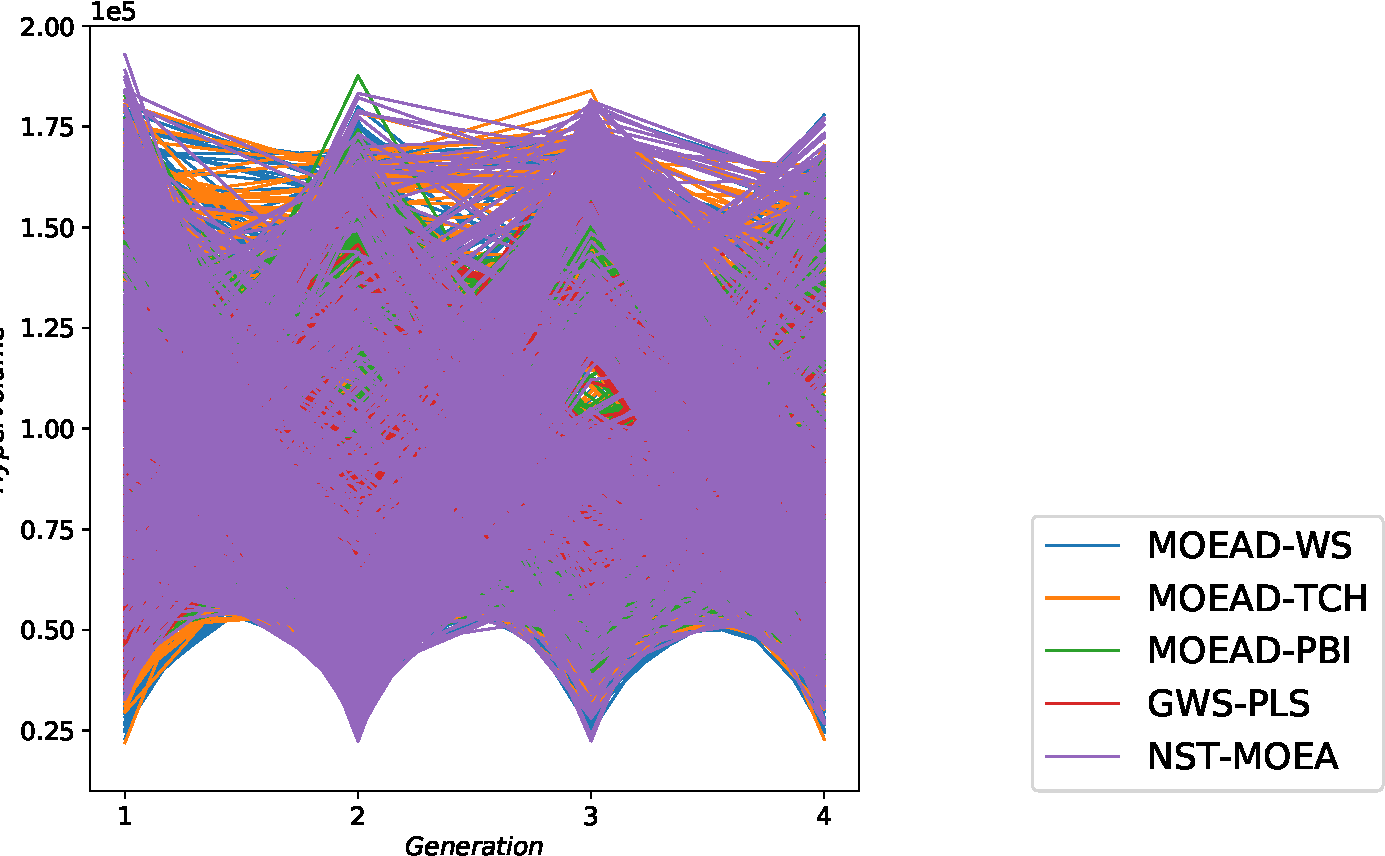
\includegraphics[width=.5\linewidth]{PF/KroAB300/Thesis-All-SameScale1-PF.pdf}} \qquad
%     \subfloat[NST-MOEA \label{subfig:KroAB300-NST-MOEA}]{\includegraphics[width=.32\linewidth]{PF/KroAB300/Thesis-NST-MOEA-SameScale1-PF.pdf}} 
%     \caption[各算法在KroAB300上的非支配解集示意图]{各算法在KroAB300上的非支配解集示意图}
%     \label{fig:各算法在KroAB300上的非支配解集示意图}
% \end{figure}
% \begin{figure}[t]
%     \ContinuedFloat
%     \subfloat[MOEA/D-WS \label{subfig:KroAB300-MOEA/D-WS}]{\includegraphics[width=.3\linewidth]{PF/KroAB300/Thesis-MOEAD-WS-SameScale1-PF.pdf}} \quad
%     \subfloat[MOEA/D-TCH \label{subfig:KroAB300-MOEA/D-TCH}]{\includegraphics[width=.3\linewidth]{PF/KroAB300/Thesis-MOEAD-TCH-SameScale1-PF.pdf}} \quad
%     \subfloat[MOEA/D-PBI \label{subfig:KroAB300-MOEA/D-PBI}]{\includegraphics[width=.3\linewidth]{PF/KroAB300/Thesis-MOEAD-PBI-SameScale1-PF.pdf}} \\
%     \subfloat[DCDG \label{subfig:KroAB300-DCDG}]{\includegraphics[width=.3\linewidth]{PF/KroAB300/Thesis-DCDG-SameScale1-PF.pdf}} \quad
%     \subfloat[GWS-PLS \label{subfig:KroAB300-GWS-PLS}]{\includegraphics[width=.3\linewidth]{PF/KroAB300/Thesis-GWS-PLS-SameScale1-PF.pdf}} \quad
%     \subfloat[2PPLS \label{subfig:KroAB300-2PPLS}]{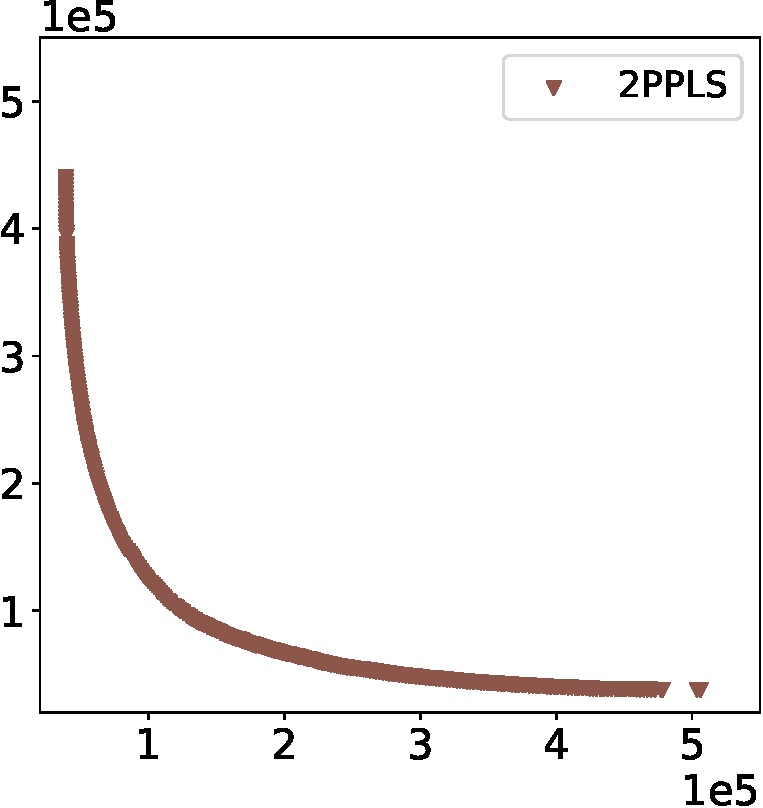
\includegraphics[width=.3\linewidth]{PF/KroAB300/Thesis-2PPLS-SameScale1-PF.pdf}}
%     \caption[]{各算法在KroAB300上的非支配解集示意图(续)}
% \end{figure}
\begin{figure}[!h]
    \subfloat[All Algorithms \label{subfig:KroAB300-All Algorithms}]{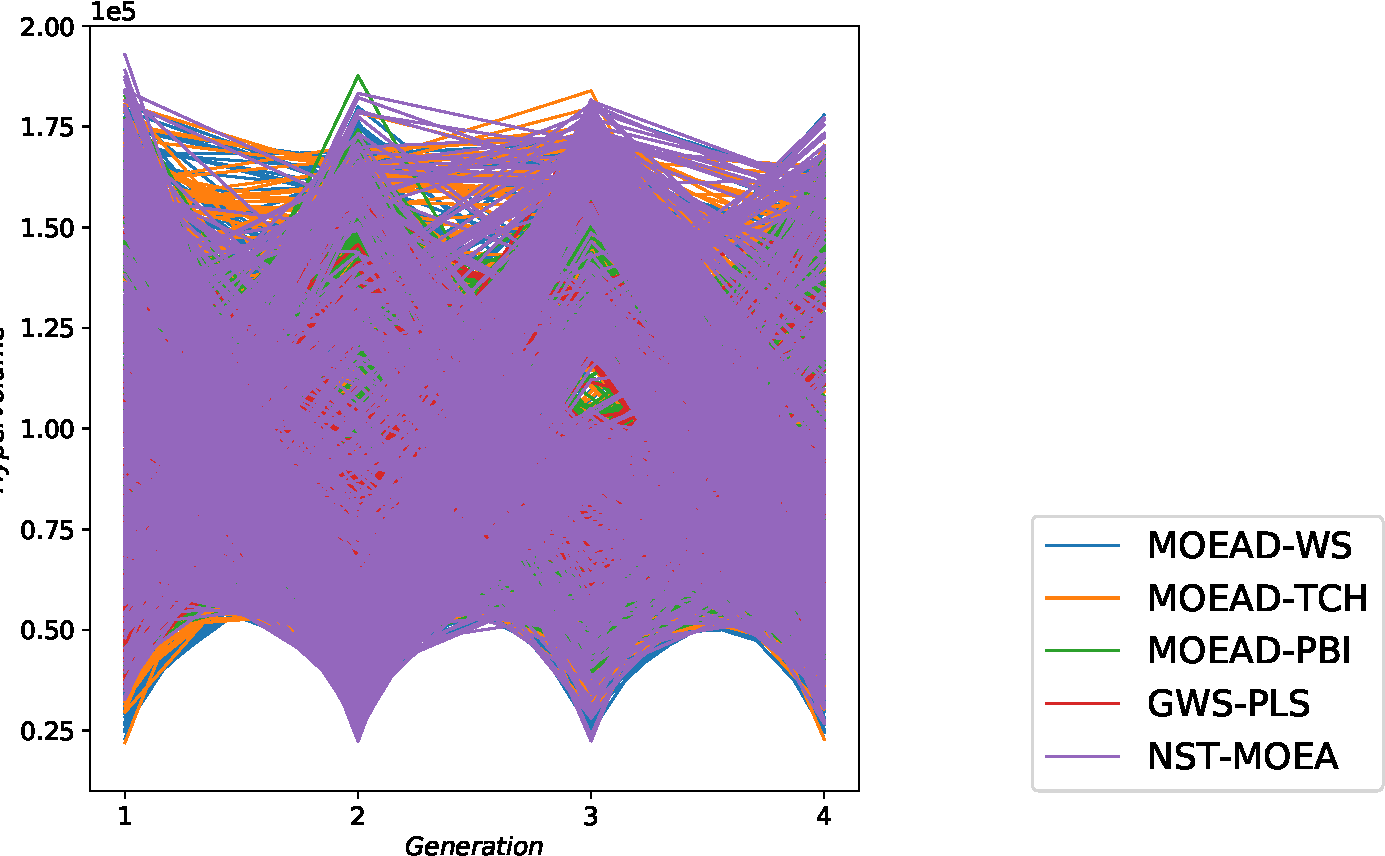
\includegraphics[width=.5\linewidth]{PF/KroAB300/Thesis-All-SameScale1-PF.pdf}} \qquad
    \subfloat[NST-MOEA \label{subfig:KroAB300-NST-MOEA}]{\includegraphics[width=.32\linewidth]{PF/KroAB300/Thesis-NST-MOEA-SameScale1-PF.pdf}}  \\
    \subfloat[MOEA/D-WS \label{subfig:KroAB300-MOEA/D-WS}]{\includegraphics[width=.3\linewidth]{PF/KroAB300/Thesis-MOEAD-WS-SameScale1-PF.pdf}} \quad
    \subfloat[MOEA/D-TCH \label{subfig:KroAB300-MOEA/D-TCH}]{\includegraphics[width=.3\linewidth]{PF/KroAB300/Thesis-MOEAD-TCH-SameScale1-PF.pdf}} \quad
    \subfloat[MOEA/D-PBI \label{subfig:KroAB300-MOEA/D-PBI}]{\includegraphics[width=.3\linewidth]{PF/KroAB300/Thesis-MOEAD-PBI-SameScale1-PF.pdf}} \\
    \subfloat[DCDG \label{subfig:KroAB300-DCDG}]{\includegraphics[width=.3\linewidth]{PF/KroAB300/Thesis-DCDG-SameScale1-PF.pdf}} \quad
    \subfloat[GWS-PLS \label{subfig:KroAB300-GWS-PLS}]{\includegraphics[width=.3\linewidth]{PF/KroAB300/Thesis-GWS-PLS-SameScale1-PF.pdf}} \quad
    \subfloat[2PPLS \label{subfig:KroAB300-2PPLS}]{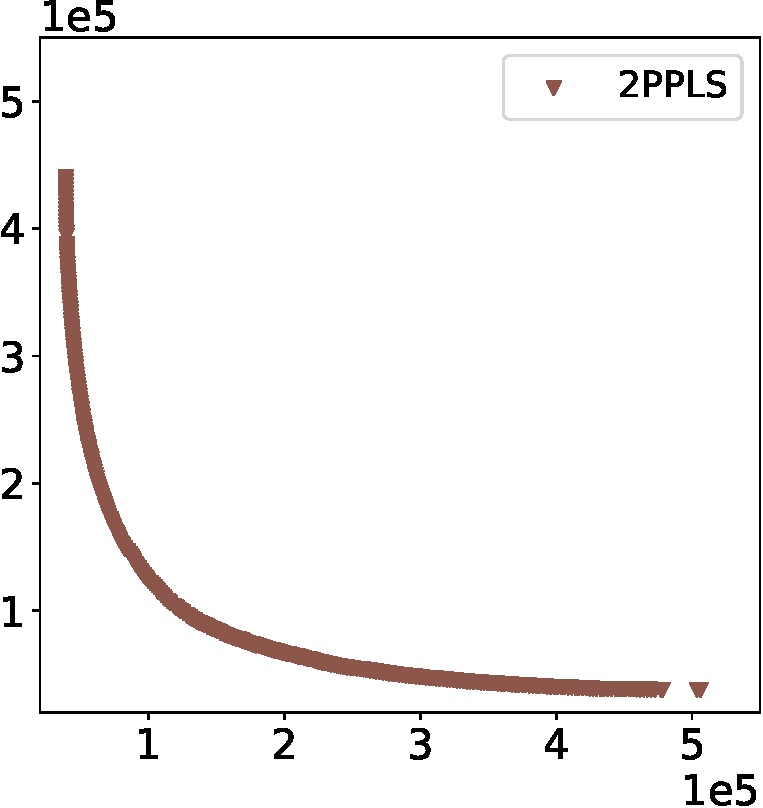
\includegraphics[width=.3\linewidth]{PF/KroAB300/Thesis-2PPLS-SameScale1-PF.pdf}}
    \caption[各算法在KroAB300上的非支配解集示意图]{各算法在KroAB300上的非支配解集示意图}
    \label{fig:各算法在KroAB300上的非支配解集示意图}
\end{figure}
\par
从\autoref{fig:各算法在KroAB300上的非支配解集示意图}~可以看出,在二目标测试问题上,MOEA/D-WS得到的非支配解集分布广泛但是不均匀,其PF面有很多缺失的部分。相反,MOEA/D-TCH和MOEA/D-PBI得到的非支配解集分布均匀但是不广泛,丢失了两端边界区域的解,可以看出,子问题不同的分解方式对MOEA/D最终的非支配解集的影响会很大。DCDG获得的非支配解集与MOEA/D-PBI类似,相比于其他算法,它也缺失了两端边界区域的解。从图中还能看出,GWS-PLS、2PPLS和NST-MOEA获得的非支配解集都分布广泛且均匀,但是在最后一个子图的局部放大图中可以看出,NST-MOEA获得的非支配解集的收敛效果比其他算法都好。从\autoref{fig:各算法在KroABC100上的非支配解集示意图}~和\autoref{fig:各算法在KroABCD100上的非支配解集示意图}~可以看出,各算法在高维目标测试问题与二目标测试问题所呈现的非支配解集分布情况相似。除了NST-MOEA获得的非支配解集分布广泛且均匀,MOEA/D-LS获得的解集广泛但不均匀外,其他算法获得的解集都在不同程度上缺失了边界区域的解。并且,结合\autoref{fig:各算法Hypervolume指标对比示意图}~所示的各算法HV指标箱型图,能够知道,NST-MOEA在获得的非支配解集不仅在分布性上表现的要比其他算法好,而且非支配解集的收敛性也要由于其他算法。
\begin{figure}[!h]
    \subfloat[NST-MOEA \label{subfig:KroABC100-NST-MOEA}]{\includegraphics[width=.275\linewidth]{PF/KroABC100/Thesis-NST-MOEA-SameScale1-PF.pdf}} \quad
    \subfloat[MOEA/D-WS \label{subfig:KroABC100-MOEA/D-WS}]{\includegraphics[width=.275\linewidth]{PF/KroABC100/Thesis-MOEAD-WS-SameScale1-PF.pdf}} \quad
    \subfloat[MOEA/D-TCH \label{subfig:KroABC100-MOEA/D-TCH}]{\includegraphics[width=.275\linewidth]{PF/KroABC100/Thesis-MOEAD-TCH-SameScale1-PF.pdf}} \\
    \subfloat[MOEA/D-PBI \label{subfig:KroABC100-MOEA/D-PBI}]{\includegraphics[width=.275\linewidth]{PF/KroABC100/Thesis-MOEAD-PBI-SameScale1-PF.pdf}} \quad
    \subfloat[DCDG \label{subfig:KroABC100-DCDG}]{\includegraphics[width=.275\linewidth]{PF/KroABC100/Thesis-DCDG-SameScale1-PF.pdf}}  \quad
    \subfloat[GWS-PLS \label{subfig:KroABC100-GWS-PLS}]{\includegraphics[width=.275\linewidth]{PF/KroABC100/Thesis-GWS-PLS-SameScale1-PF.pdf}}
    \caption[各算法在KroABC100上的非支配解集示意图]{各算法在KroABC100上的非支配解集示意图}
    \label{fig:各算法在KroABC100上的非支配解集示意图}
\end{figure}
\begin{figure}[!h]
    \subfloat[MOEA/D-WS \label{subfig:KroABCD100-MOEA/D-WS}]{\includegraphics[width=.275\linewidth]{PF/KroABCD100/Thesis-MOEAD-WS-SameScale1-PF.pdf}} \quad
    \subfloat[MOEA/D-TCH \label{subfig:KroABCD100-MOEA/D-TCH}]{\includegraphics[width=.275\linewidth]{PF/KroABCD100/Thesis-MOEAD-TCH-SameScale1-PF.pdf}} \quad
    \subfloat[MOEA/D-PBI \label{subfig:KroABCD100-MOEA/D-PBI}]{\includegraphics[width=.275\linewidth]{PF/KroABCD100/Thesis-MOEAD-PBI-SameScale1-PF.pdf}} \\
    \subfloat[GWS-PLS \label{subfig:KroABCD100-GWS-PLS}]{\includegraphics[width=.275\linewidth]{PF/KroABCD100/Thesis-GWS-PLS-SameScale1-PF.pdf}} \quad
    \subfloat[NST-MOEA \label{subfig:KroABCD100-NST-MOEA}]{\includegraphics[width=.275\linewidth]{PF/KroABCD100/Thesis-NST-MOEA-SameScale1-PF.pdf}}
    \caption[各算法在KroABCD100上的非支配解集示意图]{各算法在KroABCD100上的非支配解集示意图}
    \label{fig:各算法在KroABCD100上的非支配解集示意图}
\end{figure}
\begin{figure}[!h]
    \subfloat[KroAB100 \label{subfig:Box-HV-kroAB100}]{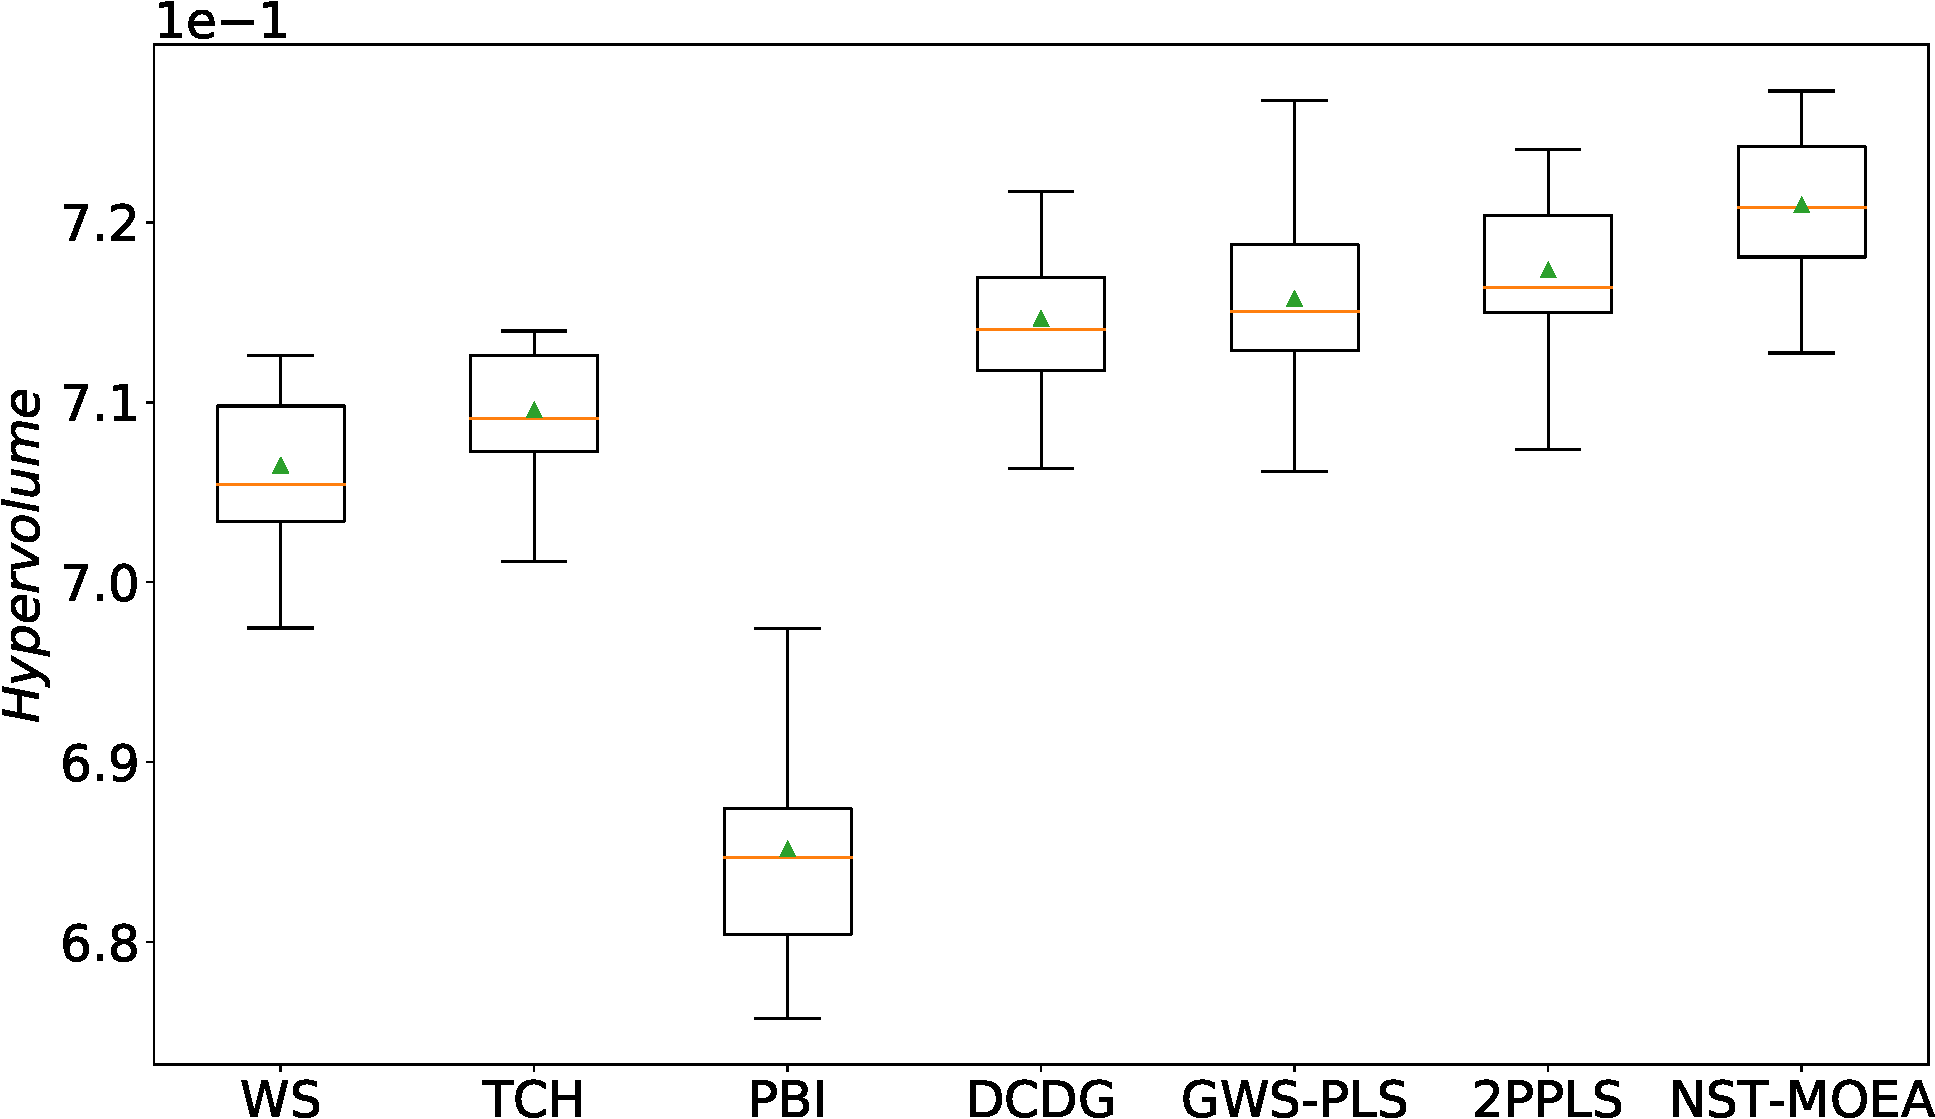
\includegraphics[width=.4\linewidth]{Box-HV-KroAB100.pdf}} \quad
    \subfloat[KroAB300 \label{subfig:Box-HV-kroAB300}]{\includegraphics[width=.4\linewidth]{Box-HV-KroAB300.pdf}} \\
    \subfloat[KroABC100 \label{subfig:Box-HV-KroABC100}]{\includegraphics[width=.4\linewidth]{Box-HV-KroABC100.pdf}} \quad
    \subfloat[KroABCD100 \label{subfig:Box-HV-KroABCD100}]{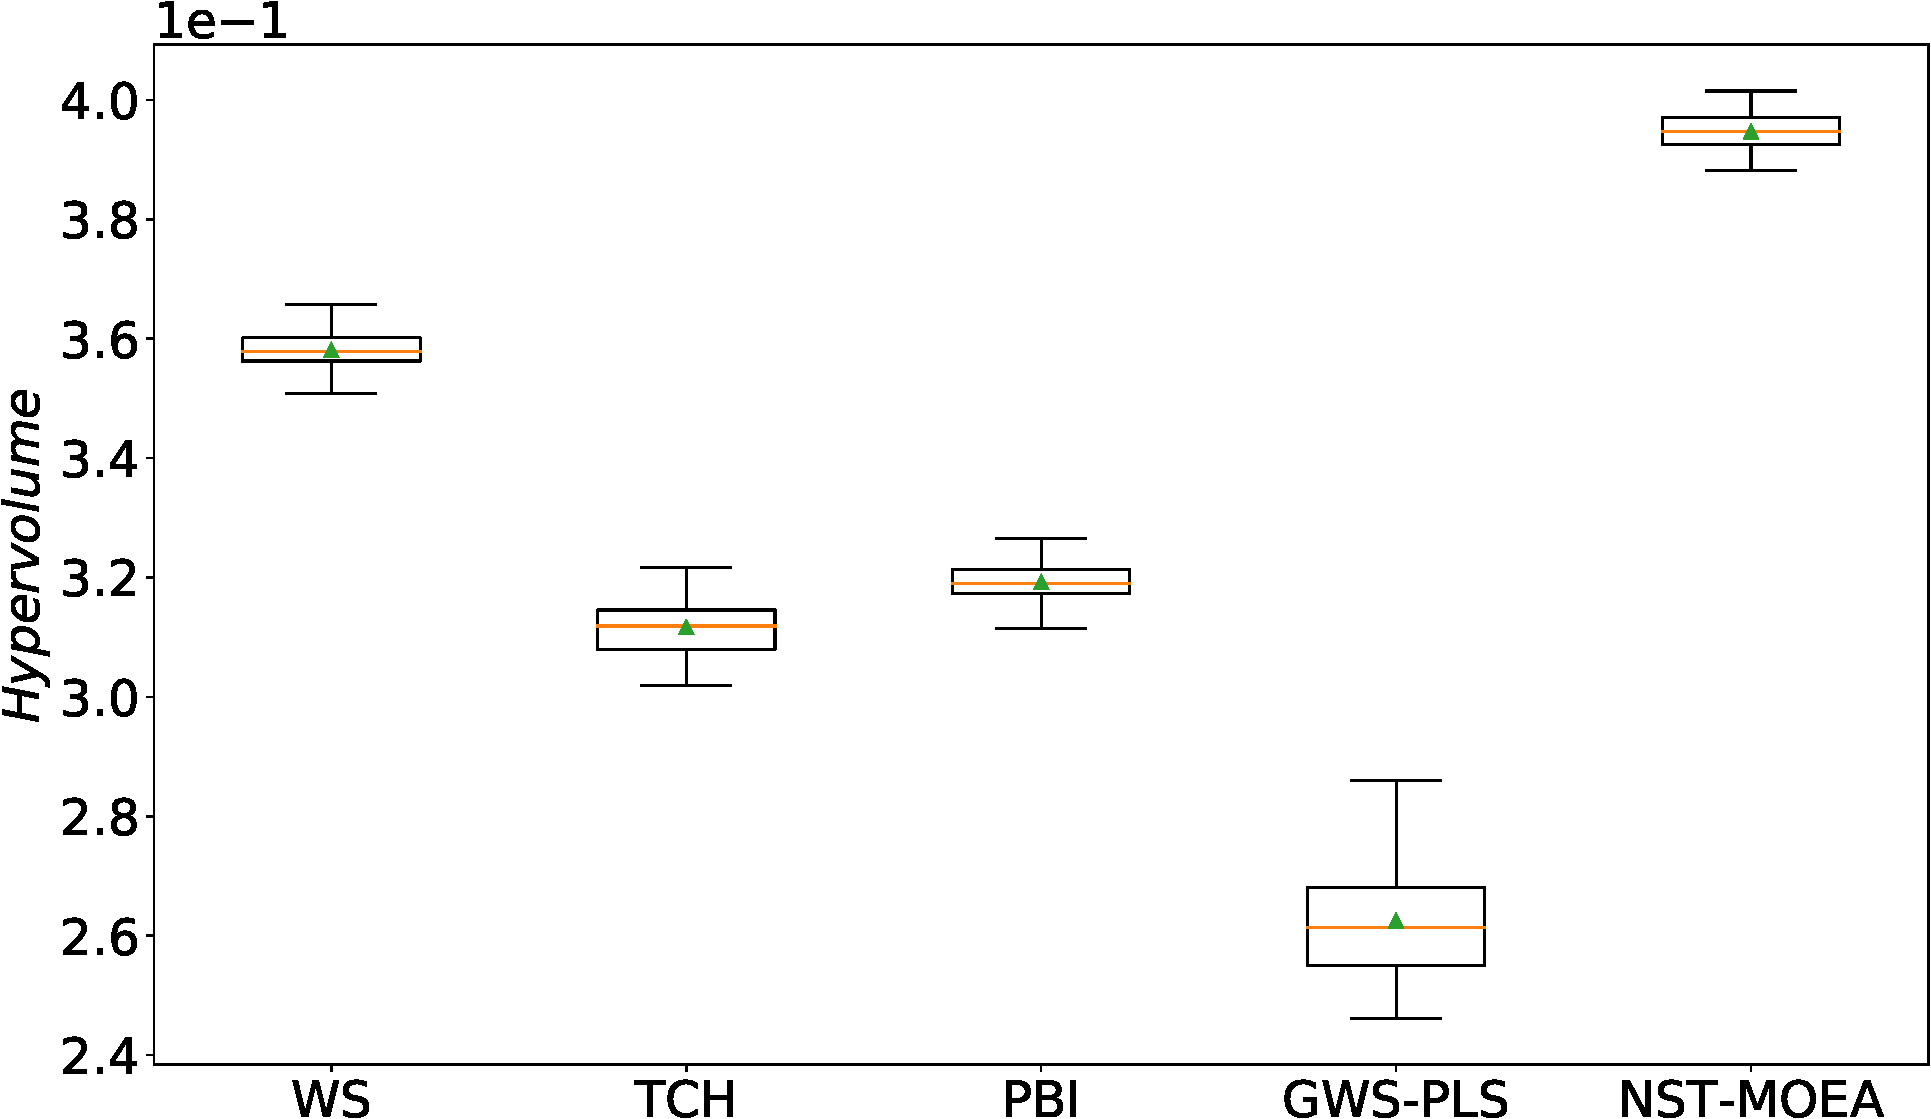
\includegraphics[width=.4\linewidth]{Box-HV-KroABCD100.pdf}}
    \caption[各算法Hypervolume指标对比示意图]{各算法Hypervolume指标对比示意图}
    \label{fig:各算法Hypervolume指标对比示意图}
\end{figure}
\par
为了更进一步地了解算法在TSPLIB测试用例的表现,现将各算法在所有TSPLIB测试用例上运行30次所获得的非支配解集的Hypervolume指标和C-Metric指标进行对比。\autoref{tab:各算法在TSPLIB测试集上获得的非支配解集的Hypervolume指标对比}~展现的是各算法在测试用例上所获得的非支配解集的Hypervolume指标,从\autoref{tab:各算法在TSPLIB测试集上获得的非支配解集的Hypervolume指标对比}~中能够看出,NST-MOEA获得的非支配解集在Hypervolume指标上要显著优于其他对比的算法,并且Hypervolume指标能够反映解集的综合性能,由此可说明NST-MOEA获得的质量要比其他对比算法要好。同时,在\autoref{tab:各算法在TSPLIB测试集上获得的非支配解集的C-Metric指标对比}~中展现的是各算法在三目标以下的测试用例上所获得的非支配解集的C-Metric指标,从\autoref{tab:各算法在TSPLIB测试集上获得的非支配解集的C-Metric指标对比}~中能够看出,NST-MOEA获得的非支配解集在一些测试用例上几乎要完全支配其他算法获得的非支配解集,并且C-Metric指标能够反映解集的收敛情况,由此可说明NST-MOEA能够获得比其他算法收敛性更好的非支配解集。
{\small
\setlength{\tabcolsep}{4.5pt}
\renewcommand\arraystretch{.65}
\begin{longtable}[c]{lccccccc}
    \caption{各算法在TSPLIB测试集上获得的非支配解集的Hypervolume指标对比}\label{tab:各算法在TSPLIB测试集上获得的非支配解集的Hypervolume指标对比}\\
    \toprule
    \multirow{2}[4]{*}{测试用例} & \multicolumn{3}{c}{MOEA/D} & \multicolumn{1}{c}{\multirow{2}[4]{*}{DCDG}} & \multicolumn{1}{c}{\multirow{2}[4]{*}{GWS-PLS}} & \multicolumn{1}{c}{\multirow{2}[4]{*}{2PPLS}} & \multicolumn{1}{c}{\multirow{2}[4]{*}{NST-MOEA}} \\
    \cmidrule{2-4}          & \multicolumn{1}{c}{WS} & \multicolumn{1}{c}{THC} & \multicolumn{1}{c}{PBI} &       &       &       &  \\
    \midrule
    \endfirsthead
    \multicolumn{8}{c}{\nuaafontcaption 续表~\thetable\hskip1em 各算法在TSPLIB测试集上获得的非支配解集的Hypervolume指标对比}\\
    \toprule
    \multirow{2}[4]{*}{测试用例} & \multicolumn{3}{c}{MOEA/D} & \multicolumn{1}{c}{\multirow{2}[4]{*}{DCDG}} & \multicolumn{1}{c}{\multirow{2}[4]{*}{GWS-PLS}} & \multicolumn{1}{c}{\multirow{2}[4]{*}{2PPLS}} & \multicolumn{1}{c}{\multirow{2}[4]{*}{NST-MOEA}} \\
    \cmidrule{2-4}          & \multicolumn{1}{c}{WS} & \multicolumn{1}{c}{THC} & \multicolumn{1}{c}{PBI} &       &       &       &  \\
    \midrule
    \endhead
    \hline
    \multicolumn{8}{r}{续下页} \\
    \endfoot
    \endlastfoot
    %2 obj
    %kro 
    KroAB100              & 7.082e-01$^{\dag}$ & 7.110e-01$^{\dag}$ & 6.867e-01$^{\dag}$ & 7.163e-01$^{\dag}$ & 7.170e-01$^{\dag}$ & 7.190e-01$^{\dag}$ & \textbf{7.226e-01} \\
                                           & 3.8e-03            & 3.7e-03            & 4.8e-03            & 4.3e-03            & 3.9e-03            & 3.7e-03            & 3.6e-03            \\
    \midrule
    KroAB200             & 7.708e-01$^{\dag}$ & 7.629e-01$^{\dag}$ & 7.396e-01$^{\dag}$ & 7.781e-01$^{\dag}$ & 7.743e-01$^{\dag}$ & 7.794e-01$^{\dag}$ & \textbf{7.837e-01} \\
                                            & 3.8e-03            & 3.9e-03            & 3.8e-03            & 3.1e-03            & 3.8e-03            & 3.4e-03            & 3.4e-03            \\
    \midrule
    KroAB300             & 8.015e-01$^{\dag}$ & 7.805e-01$^{\dag}$ & 7.667e-01$^{\dag}$ & 8.055e-01$^{\dag}$ & 8.007e-01$^{\dag}$ & 8.089e-01$^{\dag}$  & \textbf{8.129e-01} \\
                                        & 1.3e-03            & 3.6e-03            & 2.4e-03            & 2.8e-03            & 1.7e-03            & 1.4e-03                        & 1.3e-03            \\
    \midrule
    KroAB400             & 8.166e-01$^{\dag}$ & 7.863e-01$^{\dag}$ & 7.805e-01$^{\dag}$ & 8.189e-01$^{\dag}$ & 8.085e-01$^{\dag}$ & 8.229e-01$^{\dag}$  & \textbf{8.273e-01} \\
                                                & 1.3e-03            & 2.5e-03            & 2.3e-03            & 4.2e-03            & 1.9e-03            & 1.2e-03                         & 1.2e-03            \\
    \midrule
    KroAB500             & 8.309e-01$^{\dag}$ & 7.969e-01$^{\dag}$ & 7.959e-01$^{\dag}$ & 8.305e-01$^{\dag}$ & 8.267e-01$^{\dag}$ & 8.360e-01$^{\dag}$  & \textbf{8.418e-01} \\
                                            & 1.4e-03            & 3.1e-03            & 2.4e-03            & 3.9e-03            & 1.4e-03            & 1.2e-03                       & 1.2e-03            \\
    \midrule
    KroAB750          & 8.594e-01$^{\dag}$ & 8.118e-01$^{\dag}$ & 8.224e-01$^{\dag}$ & 8.576e-01$^{\dag}$ & 8.513e-01$^{\dag}$ & 8.605e-01$^{\dag}$  & \textbf{8.682e-01} \\
                                            & 1.2e-03            & 2.7e-03            & 1.5e-03            & 4.9e-03            & 7.3e-03            & 9.6e-04                       & 9.3e-04            \\
    \midrule
    KroAB1000              & 8.757e-01$^{\dag}$ & 8.194e-01$^{\dag}$ & 8.392e-01$^{\dag}$ & 8.755e-01$^{\dag}$ & 8.388e-01$^{\dag}$ & 8.749e-01$^{\dag}$  & \textbf{8.818e-01} \\
                                            & 7.8e-04            & 2.4e-03            & 1.5e-03            & 3.9e-03            & 2.9e-02            & 8.5e-04                      & 6.8e-04            \\
    \midrule

    %cluster
    ClusterAB100         & 7.250e-01$^{\dag}$ & 7.276e-01$^{\dag}$ & 6.913e-01$^{\dag}$ & 7.312e-01$^{\dag}$ & 7.312e-01$^{\dag}$ & 7.318e-01$^{\dag}$ & \textbf{7.355e-01} \\
                                                & 3.2e-03            & 3.0e-03            & 3.0e-03            & 3.1e-03            & 3.1e-03            & 3.0e-03                      & 3.1e-03            \\
    \midrule
    ClusterAB300        & 8.244e-01$^{\dag}$ & 8.077e-01$^{\dag}$ & 7.899e-01$^{\dag}$ & 8.303e-01$^{\dag}$ & 8.250e-01$^{\dag}$ & 8.323e-01$^{\dag}$  & \textbf{8.349e-01} \\
                                            & 3.1e-03            & 2.8e-03            & 2.9e-03            & 3.5e-03            & 2.7e-03            & 2.6e-03                        & 2.4e-03            \\
    \midrule
    ClusterAB500          & 8.722e-01$^{\dag}$ & 8.443e-01$^{\dag}$ & 8.335e-01$^{\dag}$ & 8.717e-01$^{\dag}$ & 8.473e-01$^{\dag}$ & 8.746e-01$^{\dag}$ & \textbf{8.806e-01} \\
                                            & 1.3e-03            & 2.5e-03            & 1.3e-03            & 3.9e-03            & 1.1e-01            & 1.1e-03                        & 1.1e-03            \\
    \midrule

    %euclid
    EuclidAB100          & 6.399e-01$^{\dag}$ & 6.480e-01$^{\dag}$ & 6.237e-01$^{\dag}$ & 6.544e-01$^{\dag}$ & 6.542e-01$^{\dag}$ & 6.562e-01$^{\dag}$  & \textbf{6.600e-01} \\
                                            & 4.5e-03            & 4.0e-03            & 5.3e-03            & 3.6e-03            & 3.9e-03            & 3.9e-03                         & 3.7e-03            \\
    \midrule
    EuclidAB300           & 7.704e-01$^{\dag}$ & 7.508e-01$^{\dag}$ & 7.414e-01$^{\dag}$ & 7.747e-01$^{\dag}$ & 7.715e-01$^{\dag}$ & 7.799e-01$^{\dag}$  & \textbf{7.844e-01} \\
                                            & 2.9e-03            & 5.2e-03            & 3.3e-03            & 3.1e-03            & 3.3e-03            & 2.9e-03                         & 2.8e-03            \\
    \midrule
    EuclidAB500         & 8.155e-01$^{\dag}$ & 7.790e-01$^{\dag}$ & 7.821e-01$^{\dag}$ & 8.140e-01$^{\dag}$ & 8.111e-01$^{\dag}$ & 8.206e-01$^{\dag}$  & \textbf{8.277e-01} \\
                                        & 9.8e-04            & 2.7e-03            & 1.7e-03            & 4.4e-03            & 1.7e-03            & 9.3e-04                         & 8.7e-04            \\
    \midrule

    %3 obj
    KroABC100             & 5.382e-01$^{\dag}$ & 5.167e-01$^{\dag}$ & 4.967e-01$^{\dag}$ & 4.925e-01$^{\dag}$ & 4.856e-01$^{\dag}$ & N.A.                 & \textbf{5.630e-01} \\
                                            & 3.8e-03            & 4.3e-03            & 4.3e-03            & 4.1e-03            & 9.4e-03            & N.A.                        & 3.5e-03            \\
    \midrule
    KroBCD100            & 5.243e-01$^{\dag}$ & 5.026e-01$^{\dag}$ & 4.837e-01$^{\dag}$ & 4.806e-01$^{\dag}$ & 4.745e-01$^{\dag}$ & N.A.                  & \textbf{5.489e-01} \\
                                            & 3.3e-03            & 3.5e-03            & 4.4e-03            & 4.7e-03            & 8.9e-03            & N.A.                           & 3.4e-03            \\
    \midrule
    KroCDE100             & 5.445e-01$^{\dag}$ & 5.227e-01$^{\dag}$ & 5.028e-01$^{\dag}$ & 4.962e-01$^{\dag}$ & 4.928e-01$^{\dag}$ & N.A.                & \textbf{5.686e-01} \\
                                            & 5.3e-03            & 5.8e-03            & 5.4e-03            & 6.5e-03            & 9.7e-03            & N.A.                           & 5.3e-03            \\
    \midrule
    %4 obj
    KroA$\sim$D100          & 3.596e-01$^{\dag}$ & 3.137e-01$^{\dag}$ & 3.207e-01$^{\dag}$ & N.A.               & 2.635e-01$^{\dag}$ & N.A.                 & \textbf{3.960e-01} \\
                                            & 3.4e-03            & 4.4e-03            & 3.7e-03            & N.A.               & 9.3e-03            & N.A.                            & 3.3e-03            \\
    \midrule
    KroB$\sim$E100         & 3.818e-01$^{\dag}$ & 3.383e-01$^{\dag}$ & 3.404e-01$^{\dag}$ & N.A.               & 2.845e-01$^{\dag}$ & N.A.                  & \textbf{4.163e-01} \\
                                            & 4.1e-03            & 4.6e-03            & 3.7e-03            & N.A.               & 1.2e-02            & N.A.                           & 3.4e-03            \\
    \midrule
    EuclidA$\sim$D100        & 2.948e-01$^{\dag}$ & 2.519e-01$^{\dag}$ & 2.610e-01$^{\dag}$ & N.A.               & 2.185e-01$^{\dag}$ & N.A.                 & \textbf{3.778e-01} \\
                                            & 5.4e-03            & 6.0e-03            & 4.8e-03            & N.A.               & 1.0e-02            & N.A.                            & 4.8e-03            \\
    \midrule
    EuclidB$\sim$E100         & 2.823e-01$^{\dag}$ & 2.428e-01$^{\dag}$ & 2.529e-01$^{\dag}$ & N.A.               & 2.071e-01$^{\dag}$ & N.A.                 & \textbf{3.714e-01} \\
                                            & 3.7e-03            & 4.6e-03            & 3.6e-03            & N.A.               & 7.4e-03            & N.A.                            & 3.0e-03            \\
    \midrule
    EuclidC$\sim$F100       & 2.842e-01$^{\dag}$ & 2.448e-01$^{\dag}$ & 2.531e-01$^{\dag}$ & N.A.               & 2.067e-01$^{\dag}$ & N.A.                 & \textbf{3.270e-01} \\
                                            & 2.6e-03            & 3.7e-03            & 2.8e-03            & N.A.               & 7.2e-03            & N.A.                           & 2.6e-03            \\
    \midrule
    EuclidD$\sim$G100       & 2.973e-01$^{\dag}$ & 2.549e-01$^{\dag}$ & 2.625e-01$^{\dag}$ & N.A.               & 2.170e-01$^{\dag}$ & N.A.                  & \textbf{3.363e-01} \\
                                            & 3.7e-03            & 4.2e-03            & 3.6e-03            & N.A.               & 8.7e-03            & N.A.                             & 3.7e-03            \\
    \midrule
    EuclidE$\sim$H100        & 2.844e-01$^{\dag}$ & 2.429e-01$^{\dag}$ & 2.520e-01$^{\dag}$ & N.A.               & 2.067e-01$^{\dag}$ & N.A.                  & \textbf{3.251e-01} \\
                                            & 3.1e-03            & 4.4e-03            & 3.1e-03            & N.A.               & 6.3e-03            & N.A.                            & 3.1e-03            \\
    \midrule

    %5 obj
    EuclidA$\sim$E100        & 1.587e-01$^{\dag}$ & 1.204e-01$^{\dag}$ & 1.384e-01$^{\dag}$ & N.A.               & 9.945e-02$^{\dag}$ & N.A.                   & \textbf{2.258e-01} \\
                                            & 3.2e-03            & 2.8e-03            & 2.6e-03            & N.A.               & 4.2e-03            & N.A.                            & 2.8e-03            \\
    \midrule
    EuclidB$\sim$F100       & 1.559e-01$^{\dag}$ & 1.196e-01$^{\dag}$ & 1.364e-01$^{\dag}$ & N.A.               & 9.800e-02$^{\dag}$ & N.A.                & \textbf{2.213e-01} \\
                                            & 3.0e-03            & 3.5e-03            & 2.6e-03            & N.A.               & 3.8e-03            & N.A.            & 2.6e-03            \\
    \midrule
    EuclidC$\sim$G100        & 1.610e-01$^{\dag}$ & 1.243e-01$^{\dag}$ & 1.421e-01$^{\dag}$ & N.A.               & 9.913e-02$^{\dag}$ & N.A.              & \textbf{2.027e-01} \\
                                            & 3.8e-03            & 3.9e-03            & 3.0e-03            & N.A.               & 5.0e-03            & N.A.            & 3.6e-03            \\
    \midrule
    EuclidD$\sim$H100       & 1.655e-01$^{\dag}$ & 1.282e-01$^{\dag}$ & 1.448e-01$^{\dag}$ & N.A.               & 1.041e-01$^{\dag}$ & N.A.             & \textbf{2.019e-01} \\
                                            & 2.5e-03            & 3.3e-03            & 2.0e-03            & N.A.               & 4.8e-03            & N.A.            & 2.5e-03            \\
    \midrule

    %6 obj
    EuclidA$\sim$F100      & 8.149e-02$^{\dag}$ & 5.843e-02$^{\dag}$ & 6.774e-02$^{\dag}$ & N.A.               & 4.538e-02$^{\dag}$ & N.A.              & \textbf{1.252e-01} \\
                                            & 2.3e-03            & 2.2e-03            & 1.7e-03            & N.A.               & 2.6e-03            & N.A.            & 2.5e-03            \\
    \midrule
    EuclidB$\sim$G100        & 8.203e-02$^{\dag}$ & 6.019e-02$^{\dag}$ & 6.908e-02$^{\dag}$ & N.A.               & 4.374e-02$^{\dag}$ & N.A.              & \textbf{1.301e-01} \\
                                            & 1.8e-03            & 1.8e-03            & 1.1e-03            & N.A.               & 1.9e-03            & N.A.            & 1.8e-03            \\
    \midrule
    EuclidC$\sim$H100       & 8.073e-02$^{\dag}$ & 5.856e-02$^{\dag}$ & 6.835e-02$^{\dag}$ & N.A.               & 4.354e-02$^{\dag}$ & N.A.             & \textbf{1.108e-01} \\
                                            & 1.7e-03            & 2.2e-03            & 1.2e-03            & N.A.               & 1.6e-03            & N.A.            & 2.3e-03            \\
    \midrule

    %7 obj
    EuclidA$\sim$G100      & 3.343e-02$^{\dag}$ & 2.355e-02$^{\dag}$ & 2.906e-02$^{\dag}$ & N.A.               & 1.607e-02$^{\dag}$ & N.A.             & \textbf{5.973e-02} \\
                                            & 8.9e-04            & 1.0e-03            & 6.1e-04            & N.A.               & 8.8e-04            & N.A.            & 1.1e-03            \\
    \midrule
    EuclidB$\sim$H100       & 3.501e-02$^{\dag}$ & 2.453e-02$^{\dag}$ & 2.941e-02$^{\dag}$ & N.A.               & 1.600e-02$^{\dag}$ & N.A.             & \textbf{6.211e-02} \\
                                            & 8.6e-04            & 8.9e-04            & 5.5e-04            & N.A.               & 1.1e-03            & N.A.            & 1.1e-03            \\
    % \midrule

    %8 obj
    % EuclidA$\sim$H100     & 1.578e-02$^{\dag}$ & 1.080e-02$^{\dag}$ & 1.249e-02$^{\dag}$ & N.A.               & 4.168e-03$^{\dag}$ & N.A.            & \textbf{3.081e-02} \\
    %                                         & 5.2e-04            & 4.2e-04            & 2.9e-04            & N.A.               & 6.9e-04            & N.A.            & 6.5e-04            \\
    \bottomrule
    \multicolumn{8}{p{45em}}{
        对Hypervolume指标值进行显著性水平为0.05的Wilcoxon秩和检验\vspace{-.75em}\newline{}
        $^\ddag$表示该算法在此问题解集上的Hypervolume指标显著优于NST-MOEA\vspace{-.75em}\newline{}
        $^\dag$表示该算法在此问题解集上的Hypervolume指标显著劣于NST-MOEA\vspace{-.75em}\newline{}
        $^\approx$表示该算法在此问题解集上的Hypervolume指标与NST-MOEA没有明显差异\vspace{-.75em}\newline{}
        N.A.表示该算法在合理的时间内无法获取该问题的非支配解集\vspace{-.75em}\newline{}
        每一行中,上面的数据为算法运行30次获取的Hypervolume指标的均值,下面的数据为标准差
        }
\end{longtable}
}% 设置字体大小,设置块
{
\small
% \renewcommand\arraystretch{1.2}
% \renewcommand\tabcolsep{2pt}
\setlength{\tabcolsep}{2pt}
\renewcommand\arraystretch{.7}
\begin{longtable}[c]{lcccccccccccc}
    \caption{各算法在TSPLIB测试集上获得的非支配解集的C-Metric指标对比 \label{tab:各算法在TSPLIB测试集上获得的非支配解集的C-Metric指标对比}}\\
    \toprule
    \multirow{2}[4]{*}{测试用例} & \multicolumn{2}{c}{MOEA/D-WS} & \multicolumn{2}{c}{MOEA/D-TCH} & \multicolumn{2}{c}{MOEA/D-PBI} & \multicolumn{2}{c}{DCDG} & \multicolumn{2}{c}{GWS-PLS} & \multicolumn{2}{c}{2PPLS} \\
    \cmidrule{2-13}    & C(A,B)         & C(B,A)       & C(A,B)           & C(B,A)          & C(A,B)          & C(B,A)         & C(A,B)          & C(B,A)        & C(A,B)          & C(B,A) & C(A,B)          & C(B,A) \\
    \midrule
    \endfirsthead
    \multicolumn{13}{c}{\nuaafontcaption 续表~\thetable\hskip1em 各算法在TSPLIB测试集上获得的非支配解集的C-Metric指标对比}\\
    \toprule
    \multirow{2}[4]{*}{测试用例} & \multicolumn{2}{c}{MOEA/D-WS} & \multicolumn{2}{c}{MOEA/D-TCH} & \multicolumn{2}{c}{MOEA/D-PBI} & \multicolumn{2}{c}{DCDG} & \multicolumn{2}{c}{GWS-PLS} & \multicolumn{2}{c}{2PPLS} \\
    \cmidrule{2-13}    & C(A,B)         & C(B,A)       & C(A,B)           & C(B,A)          & C(A,B)          & C(B,A)         & C(A,B)          & C(B,A)        & C(A,B)          & C(B,A) & C(A,B)          & C(B,A) \\
    \midrule
    \endhead
    \hline
    \multicolumn{13}{r}{续下页} \\
    \endfoot
    \endlastfoot
    %2 obj
    %kro
    KroAB100                      & \textbf{98.64}                & 0.05                           & \textbf{81.44}                 & 1.84                     & \textbf{90.33}              & 0.81                      & \textbf{86.73}           & 1.99   & \textbf{94.96}  & 0.83   & \textbf{77.20}  & 4.84  \\
    %3 obj
    KroAB200                      & \textbf{99.89}                & 0.01                           & \textbf{99.67}                 & 0.03                     & \textbf{99.94}              & 0.01                      & \textbf{88.04}           & 2.69   & \textbf{99.97}  & 0.00   & \textbf{97.26}  & 1.31  \\
    KroAB300                      & \textbf{96.82}                & 0.47                           & \textbf{99.74}                 & 0.02                     & \textbf{99.62}              & 0.01                      & \textbf{96.50}           & 0.50   & \textbf{99.99}  & 0.00   & \textbf{97.85}  & 0.62  \\
    KroAB400                      & \textbf{98.92}                & 0.00                           & \textbf{99.73}                 & 0.01                     & \textbf{99.81}              & 0.01                      & \textbf{95.29}           & 0.28   & \textbf{100.00} & 0.00   & \textbf{98.32}  & 0.05  \\
    KroAB500                      & \textbf{98.92}                & 0.02                           & \textbf{99.39}                 & 0.01                     & \textbf{99.62}              & 0.00                      & \textbf{95.26}           & 0.34   & \textbf{100.00} & 0.00   & \textbf{99.29}  & 0.05  \\
    KroAB750                      & \textbf{96.92}                & 0.02                           & \textbf{99.47}                 & 0.01                     & \textbf{99.73}              & 0.00                      & \textbf{96.88}           & 0.07   & \textbf{100.00} & 0.00   & \textbf{99.92}  & 0.00  \\
    KroAB1000                     & \textbf{82.54}                & 0.25                           & \textbf{90.88}                 & 0.09                     & \textbf{97.38}              & 0.04                      & \textbf{87.72}           & 0.17   & \textbf{99.15}  & 0.01   & \textbf{98.11}  & 0.06  \\

    %cluster
    ClusterAB100                  & \textbf{84.79}                & 2.30                           & \textbf{94.21}                 & 0.89                     & \textbf{62.66}              & 4.51                      & \textbf{78.44}           & 4.03   & \textbf{91.99}  & 1.84   & \textbf{82.02}  & 6.05  \\
    ClusterAB300                  & \textbf{97.82}                & 0.20                           & \textbf{98.12}                 & 0.24                     & \textbf{99.35}              & 0.13                      & \textbf{80.10}           & 6.29   & \textbf{99.89}  & 0.01   & \textbf{95.01}  & 2.62  \\
    ClusterAB500                  & \textbf{98.26}                & 0.23                           & \textbf{98.51}                 & 0.03                     & \textbf{99.64}              & 0.01                      & \textbf{93.73}           & 0.78   & \textbf{100.00} & 0.00   & \textbf{99.78}  & 0.03  \\

    %euclid
    EuclidAB100                   & \textbf{97.39}                & 0.53                           & \textbf{87.60}                 & 4.68                     & \textbf{93.32}              & 2.44                      & \textbf{82.83}           & 10.37  & \textbf{94.09}  & 1.30   & \textbf{85.93}  & 7.81  \\
    EuclidAB300                   & \textbf{99.58}                & 0.01                           & \textbf{99.48}                 & 0.04                     & \textbf{99.82}              & 0.00                      & \textbf{95.07}           & 0.53   & \textbf{99.99}  & 0.00   & \textbf{98.58}  & 0.28  \\
    EuclidAB500                   & \textbf{99.33}                & 0.03                           & \textbf{99.00}                 & 0.03                     & \textbf{99.89}              & 0.02                      & \textbf{95.83}           & 0.32   & \textbf{100.00} & 0.00   & \textbf{99.54}  & 0.05  \\

    %3 obj
    KroABC100                     & \textbf{52.96}                & 0.62                           & \textbf{97.84}                 & 0.01                     & \textbf{91.02}              & 0.07                      & \textbf{83.20}           & 0.08   & \textbf{91.20}  & 0.02   & N.A.            & N.A.  \\
    KroBCD100                     & \textbf{57.61}                & 0.43                           & \textbf{98.72}                 & 0.01                     & \textbf{93.35}              & 0.06                      & \textbf{85.23}           & 0.06   & \textbf{88.83}  & 0.02   & N.A.            & N.A.  \\
    KroCDE100                     & \textbf{56.36}                & 0.42                           & \textbf{98.27}                 & 0.00                     & \textbf{90.24}              & 0.08                      & \textbf{83.49}           & 0.07   & \textbf{89.80}  & 0.02   & N.A.            & N.A.  \\
    \bottomrule
    \multicolumn{13}{p{45em}}{
        A 代表NST-MOEA\vspace{-.75em}\newline{}
        B 代表其他对用的算法\vspace{-.75em}\newline{}
        N.A. 意味着当前算法无法在合理时间内获取问题的非支配解集
    }
\end{longtable}
}
% \begin{tablenotes}
%     \item[] A 代表NST-MOEA
%     \item[] B 代表其他对用的算法.
%     \item[] N.A. 意味着当前算法无法在合理时间内获取问题的非支配解集.
% \end{tablenotes}

% \begin{table}[!h]
%     \small
%     \renewcommand\arraystretch{1.2}
%     \renewcommand\tabcolsep{2pt}
%     \centering
%     \caption{各算法在TSPLIB测试集上获得的非支配解集的C-Metric指标对比 \label{tab:各算法在TSPLIB测试集上获得的非支配解集的C-Metric指标对比}}
%     \begin{threeparttable}
%         \begin{tabular}{lcccccccccccc}
%             \toprule
%             \multirow{2}[4]{*}{测试用例} & \multicolumn{2}{c}{MOEA/D-WS} & \multicolumn{2}{c}{MOEA/D-TCH} & \multicolumn{2}{c}{MOEA/D-PBI} & \multicolumn{2}{c}{DCDG} & \multicolumn{2}{c}{GWS-PLS} & \multicolumn{2}{c}{2PPLS} \\
%             \cmidrule{2-13}    & C(A,B)         & C(B,A)       & C(A,B)           & C(B,A)          & C(A,B)          & C(B,A)         & C(A,B)          & C(B,A)        & C(A,B)          & C(B,A) & C(A,B)          & C(B,A) \\
%             \midrule
%             %2 obj
%             %kro
%             KroAB100                      & \textbf{98.64}                & 0.05                           & \textbf{81.44}                 & 1.84                     & \textbf{90.33}              & 0.81                      & \textbf{86.73}           & 1.99   & \textbf{94.96}  & 0.83   & \textbf{77.20}  & 4.84  \\
%             %3 obj
%             KroAB200                      & \textbf{99.89}                & 0.01                           & \textbf{99.67}                 & 0.03                     & \textbf{99.94}              & 0.01                      & \textbf{88.04}           & 2.69   & \textbf{99.97}  & 0.00   & \textbf{97.26}  & 1.31  \\
%             KroAB300                      & \textbf{96.82}                & 0.47                           & \textbf{99.74}                 & 0.02                     & \textbf{99.62}              & 0.01                      & \textbf{96.50}           & 0.50   & \textbf{99.99}  & 0.00   & \textbf{97.85}  & 0.62  \\
%             KroAB400                      & \textbf{98.92}                & 0.00                           & \textbf{99.73}                 & 0.01                     & \textbf{99.81}              & 0.01                      & \textbf{95.29}           & 0.28   & \textbf{100.00} & 0.00   & \textbf{98.32}  & 0.05  \\
%             KroAB500                      & \textbf{98.92}                & 0.02                           & \textbf{99.39}                 & 0.01                     & \textbf{99.62}              & 0.00                      & \textbf{95.26}           & 0.34   & \textbf{100.00} & 0.00   & \textbf{99.29}  & 0.05  \\
%             KroAB750                      & \textbf{96.92}                & 0.02                           & \textbf{99.47}                 & 0.01                     & \textbf{99.73}              & 0.00                      & \textbf{96.88}           & 0.07   & \textbf{100.00} & 0.00   & \textbf{99.92}  & 0.00  \\
%             KroAB1000                     & \textbf{82.54}                & 0.25                           & \textbf{90.88}                 & 0.09                     & \textbf{97.38}              & 0.04                      & \textbf{87.72}           & 0.17   & \textbf{99.15}  & 0.01   & \textbf{98.11}  & 0.06  \\

%             %cluster
%             ClusterAB100                  & \textbf{84.79}                & 2.30                           & \textbf{94.21}                 & 0.89                     & \textbf{62.66}              & 4.51                      & \textbf{78.44}           & 4.03   & \textbf{91.99}  & 1.84   & \textbf{82.02}  & 6.05  \\
%             ClusterAB300                  & \textbf{97.82}                & 0.20                           & \textbf{98.12}                 & 0.24                     & \textbf{99.35}              & 0.13                      & \textbf{80.10}           & 6.29   & \textbf{99.89}  & 0.01   & \textbf{95.01}  & 2.62  \\
%             ClusterAB500                  & \textbf{98.26}                & 0.23                           & \textbf{98.51}                 & 0.03                     & \textbf{99.64}              & 0.01                      & \textbf{93.73}           & 0.78   & \textbf{100.00} & 0.00   & \textbf{99.78}  & 0.03  \\

%             %euclid
%             EuclidAB100                   & \textbf{97.39}                & 0.53                           & \textbf{87.60}                 & 4.68                     & \textbf{93.32}              & 2.44                      & \textbf{82.83}           & 10.37  & \textbf{94.09}  & 1.30   & \textbf{85.93}  & 7.81  \\
%             EuclidAB300                   & \textbf{99.58}                & 0.01                           & \textbf{99.48}                 & 0.04                     & \textbf{99.82}              & 0.00                      & \textbf{95.07}           & 0.53   & \textbf{99.99}  & 0.00   & \textbf{98.58}  & 0.28  \\
%             EuclidAB500                   & \textbf{99.33}                & 0.03                           & \textbf{99.00}                 & 0.03                     & \textbf{99.89}              & 0.02                      & \textbf{95.83}           & 0.32   & \textbf{100.00} & 0.00   & \textbf{99.54}  & 0.05  \\

%             %3 obj
%             KroABC100                     & \textbf{52.96}                & 0.62                           & \textbf{97.84}                 & 0.01                     & \textbf{91.02}              & 0.07                      & \textbf{83.20}           & 0.08   & \textbf{91.20}  & 0.02   & N.A.            & N.A.  \\
%             KroBCD100                     & \textbf{57.61}                & 0.43                           & \textbf{98.72}                 & 0.01                     & \textbf{93.35}              & 0.06                      & \textbf{85.23}           & 0.06   & \textbf{88.83}  & 0.02   & N.A.            & N.A.  \\
%             KroCDE100                     & \textbf{56.36}                & 0.42                           & \textbf{98.27}                 & 0.00                     & \textbf{90.24}              & 0.08                      & \textbf{83.49}           & 0.07   & \textbf{89.80}  & 0.02   & N.A.            & N.A.  \\
%             \bottomrule
%         \end{tabular}
%         \begin{tablenotes}
%             \item[] A 代表NST-MOEA
%             \item[] B 代表其他对用的算法.
%             \item[] N.A. 意味着当前算法无法在合理时间内获取问题的非支配解集.
%         \end{tablenotes}
%     \end{threeparttable}
% \end{table}

\subsection{邻域结构迁移的有效性分析}
\label{subsec:NST:实验与讨论:邻域结构迁移的有效性分析}
在本节中,将通过NST-MOEA与未使用邻域结构迁移(NST)的NST-MOEA作对比,以此来验证邻域结构迁移的有效性。
\autoref{tab:HV and C-Metric}~中展示了NST-MOEA和未使用NST的NST-MOEA在TSPLIB测试集上运行30次所获得的非支配解集的Hypervolume指标和部分C-Metric指标的对比数据。从表中数据可以看出,NST-MOEA在两目标测试集上的Hypervolume指标要优于未使用NST的NST-MOEA,而且在高维目标测试集上的Hypervolume指标要显著优于未使用NST的NST-MOEA。并且从C-Metric指标的对比上能够看出,NST-MOEA获得的非支配解集的收敛程度要优于未使用NST的NST-MOEA,但是由于问题越到高维,其最终的非支配解就会越多,所以在收敛效果上的表现会不明显。
\par
{
% \small
% \setlength{\tabcolsep}{4.5pt}
\renewcommand\arraystretch{.7}
\begin{longtable}[c]{lcc|cc}
    \caption{NST-MOEA和未使用NST的NST-MOEA在TSPLIB测试集上获得的非支配解集的Hypervolume指标和部分C-Metric指标的对比} \label{tab:HV and C-Metric} \\
    \toprule
    \multirow{2}[4]{*}{测试用例} & \multicolumn{2}{c|}{HV}  & \multicolumn{2}{c}{C-Metric}      \\
    \cmidrule{2-5}                   & A    & B             &    C(A,B)    & C(B,A) \\
    \midrule
    \endfirsthead
    \multicolumn{5}{c}{\nuaafontcaption 续表~\thetable\hskip1em Hypervolume指标和部分C-Metric指标的对比}\\
    \toprule
    \multirow{2}[4]{*}{测试用例} & \multicolumn{2}{c|}{HV}         & \multicolumn{2}{c}{C-Metric}      \\
    \cmidrule{2-5} & A                              & B                    & C(A,B)         & C(B,A) \\
    \midrule
    \endhead
    \hline
    \multicolumn{5}{r}{续下页} \\
    \endfoot
    \endlastfoot
    %2 obj
    KroAB100       &\textbf{7.226e-01} (3.6e-03)    &7.215e-01 (3.6e-03)$^{\approx}$   &\textbf{29.62}  &14.48 \\
    KroAB200       &\textbf{7.837e-01} (3.4e-03)    &7.833e-01 (3.4e-03)$^{\approx}$   &\textbf{45.03}  &27.71 \\
    KroAB300       &\textbf{8.129e-01} (1.3e-03)    &8.126e-01 (1.3e-03)$^{\approx}$   &\textbf{44.62}  &29.89 \\
    KroAB400       &\textbf{8.273e-01} (1.2e-03)    &8.269e-01 (1.3e-03)$^{\approx}$   &\textbf{43.06}  &29.77 \\
    KroAB500       &\textbf{8.418e-01} (1.2e-03)    &8.414e-01 (1.2e-03)$^{\approx}$   &\textbf{41.47}  &30.89 \\
    KroAB750       &\textbf{8.682e-01} (9.3e-04)    &8.680e-01 (9.8e-04)$^{\approx}$   &\textbf{41.08}  &31.12 \\
    KroAB1000      &\textbf{8.818e-01} (6.8e-04)    &8.814e-01 (7.4e-04)$^{\approx}$   &\textbf{38.19}  &29.46 \\
    ClusterAB100   &\textbf{7.355e-01} (3.1e-03)    &7.346e-01 (3.0e-03)$^{\approx}$   &\textbf{33.26}  &20.19 \\
    ClusterAB300   &\textbf{8.349e-01} (2.4e-03)    &8.348e-01 (2.5e-03)$^{\approx}$   &\textbf{40.82}  &37.97 \\
    ClusterAB500   &\textbf{8.806e-01} (1.1e-03)    &8.802e-01 (1.1e-03)$^{\approx}$   &\textbf{45.85}  &34.40 \\
    EuclidAB100    &\textbf{6.600e-01} (3.7e-03)    &6.584e-01 (3.8e-03)$^{\approx}$   &\textbf{42.27}  &19.52 \\
    EuclidAB300    &\textbf{7.844e-01} (2.8e-03)    &7.841e-01 (2.7e-03)$^{\approx}$   &\textbf{43.01}  &30.59 \\
    EuclidAB500    &\textbf{8.277e-01} (8.7e-04)    &8.273e-01 (8.0e-04)$^{\approx}$   &\textbf{44.96}  &29.97 \\
    %3 obj
    KroABC100      &\textbf{5.630e-01} (3.5e-03)    &5.603e-01 (3.4e-03)$^{\dag}$	   &\textbf{15.68}  &14.31 \\
    KroBCD100      &\textbf{5.489e-01} (3.4e-03)    &5.462e-01 (3.4e-03)$^{\dag}$	   &\textbf{15.65}  &12.51 \\
    KroCDE100      &\textbf{5.686e-01} (5.3e-03)    &5.656e-01 (5.3e-03)$^{\dag}$	   &\textbf{16.68}  &12.19 \\
    %4 obj
    KroABCD100     &\textbf{3.960e-01} (3.3e-03)	&3.921e-01 (3.2e-03)$^{\dag}$      &N.A.            &N.A. \\ 
    KroBCDE100     &\textbf{4.163e-01} (3.4e-03)	&4.124e-01 (3.8e-03)$^{\dag}$      &N.A.            &N.A. \\	
    EuclidA$\sim$D100   &\textbf{3.778e-01} (4.8e-03)	&3.730e-01 (4.5e-03)$^{\dag}$      &N.A.            &N.A. \\	
    EuclidB$\sim$E100   &\textbf{3.714e-01} (3.0e-03)	&3.652e-01 (3.7e-03)$^{\dag}$      &N.A.            &N.A. \\	
    EuclidC$\sim$F100   &\textbf{3.270e-01} (2.6e-03)	&3.212e-01 (2.5e-03)$^{\dag}$      &N.A.            &N.A. \\	
    EuclidD$\sim$G100   &\textbf{3.363e-01} (3.7e-03)	&3.324e-01 (3.5e-03)$^{\dag}$      &N.A.            &N.A. \\	
    EuclidE$\sim$H100   &\textbf{3.251e-01} (3.1e-03)	&3.213e-01 (2.8e-03)$^{\dag}$      &N.A.            &N.A. \\
    %5 obj	
    EuclidA$\sim$E100   &\textbf{2.258e-01} (2.8e-03)	&2.185e-01 (2.7e-03)$^{\dag}$      &N.A.            &N.A. \\	
    EuclidB$\sim$F100   &\textbf{2.213e-01} (2.6e-03)	&2.146e-01 (3.2e-03)$^{\dag}$      &N.A.            &N.A. \\	
    EuclidC$\sim$G100   &\textbf{2.027e-01} (3.6e-03)	&1.956e-01 (3.8e-03)$^{\dag}$      &N.A.            &N.A. \\	
    EuclidD$\sim$H100   &\textbf{2.019e-01} (2.5e-03)	&1.960e-01 (2.6e-03)$^{\dag}$      &N.A.            &N.A. \\	
    %6 obj	
    EuclidA$\sim$F100   &\textbf{1.252e-01} (2.5e-03)	&1.194e-01 (2.7e-03)$^{\dag}$      &N.A.            &N.A. \\
    EuclidB$\sim$G100   &\textbf{1.301e-01} (1.8e-03)	&1.256e-01 (1.9e-03)$^{\dag}$      &N.A.            &N.A. \\	
    EuclidC$\sim$H100   &\textbf{1.108e-01} (2.3e-03)	&1.057e-01 (2.3e-03)$^{\dag}$      &N.A.            &N.A. \\
    %7 obj		
    EuclidA$\sim$G100   &\textbf{5.973e-02} (1.1e-03)	&5.508e-02 (1.2e-03)$^{\dag}$      &N.A.            &N.A. \\	
    EuclidB$\sim$H100   &\textbf{6.211e-02} (1.1e-03)	&5.753e-02 (1.1e-03)$^{\dag}$      &N.A.            &N.A. \\	
    \bottomrule
    \multicolumn{5}{p{35em}}{
        A代表NST-MOEA,B代表未使用NST的NST-MOEA\vspace{-.75em}\newline{}
        对Hypervolume指标值进行显著性水平为0.05的Wilcoxon秩和检验\vspace{-.75em}\newline{}
        $^\ddag$,$^\dag$和$^\approx$ 分别代表对应的算法性能显著优于,劣于或相似于NST-MOEA的性能\vspace{-.75em}\newline{}
        N.A.表示无法在合理时间内计算该指标
        }
\end{longtable}
}% 设置字体大小,设置块
% \end{tabular}
% \begin{tablenotes}
%     \item[] A代表NST-MOEA,B代表未使用NST的NST-MOEA
%     \item[] 对Hypervolume指标值进行显著性水平为0.05的Wilcoxon秩和检验
%     \item[] $^\ddag$,$^\dag$和$^\approx$ 分别代表对应的算法性能显著优于,劣于或相似于NST-MOEA的性能
%     \item[] “N.A.”表示无法在合理时间内计算该指标
% \end{tablenotes}
% \end{threeparttable}
% 此外,\autoref{fig:Convergence}~中展示了NST-MOEA和未使用NST的NST-MOEA在部分测试用例上的收敛轨迹。从图中能够看出,NST-MOEA的收敛速度比未使用NST的NST-MOEA要快,并且NST-MOEA的最终性能也要优于未使用NST的NST-MOEA。综上所述,可以证实NST的有效性。
% % TODO: 换成NST-MOEA和未使用NST的NST-MOEA对比图
% \begin{figure}[h]
%     \centering
%     \subfloat[KroAB100]{ \label{subfig:LS2}
%         \includegraphics[width=.4\linewidth]{Convergence-LS-All-RealAB100.pdf}
%     }
%     \subfloat[KroAB300]{ \label{subfig:LS3}
%         \includegraphics[width=.4\linewidth]{Convergence-LS-All-RealAB300.pdf}
%     }
%     % \hfill
%     \vspace{-1em}
%     \subfloat[KroABC100]{ \label{subfig:LS4}
%         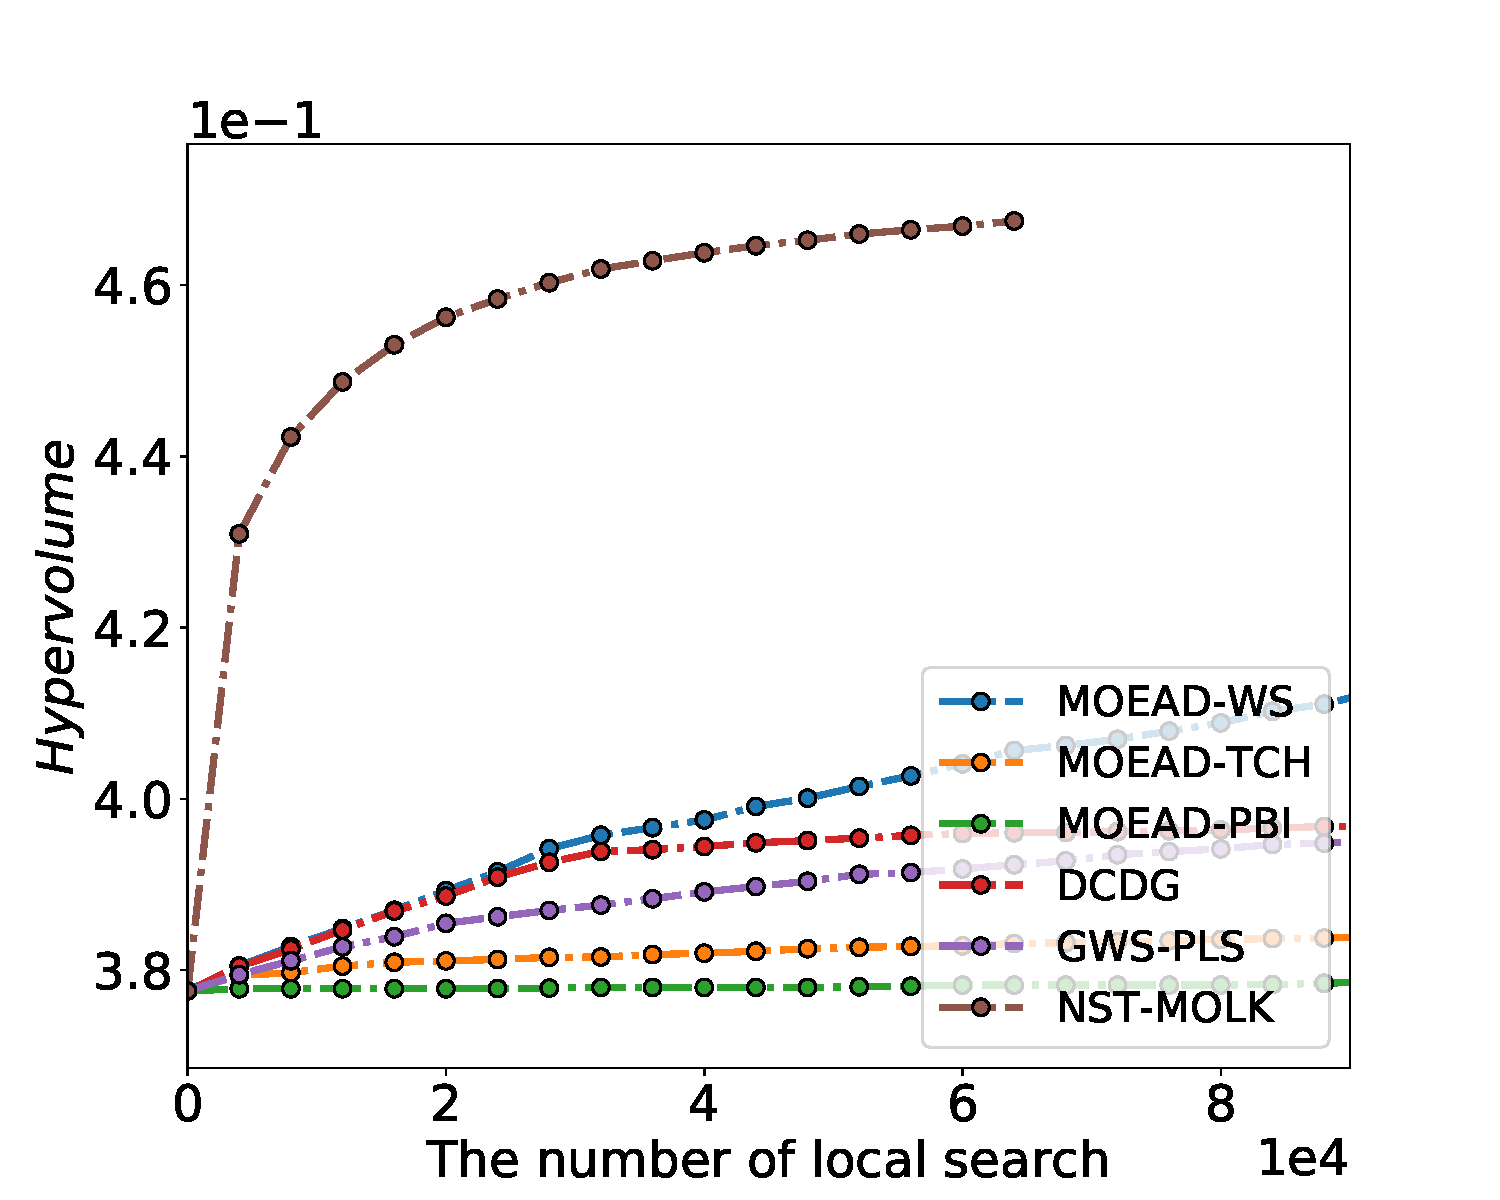
\includegraphics[width=.4\linewidth]{Convergence-LS-All-RealABC100.pdf}
%     }
%     \subfloat[KroABCD100]{ \label{subfig:LS5}
%         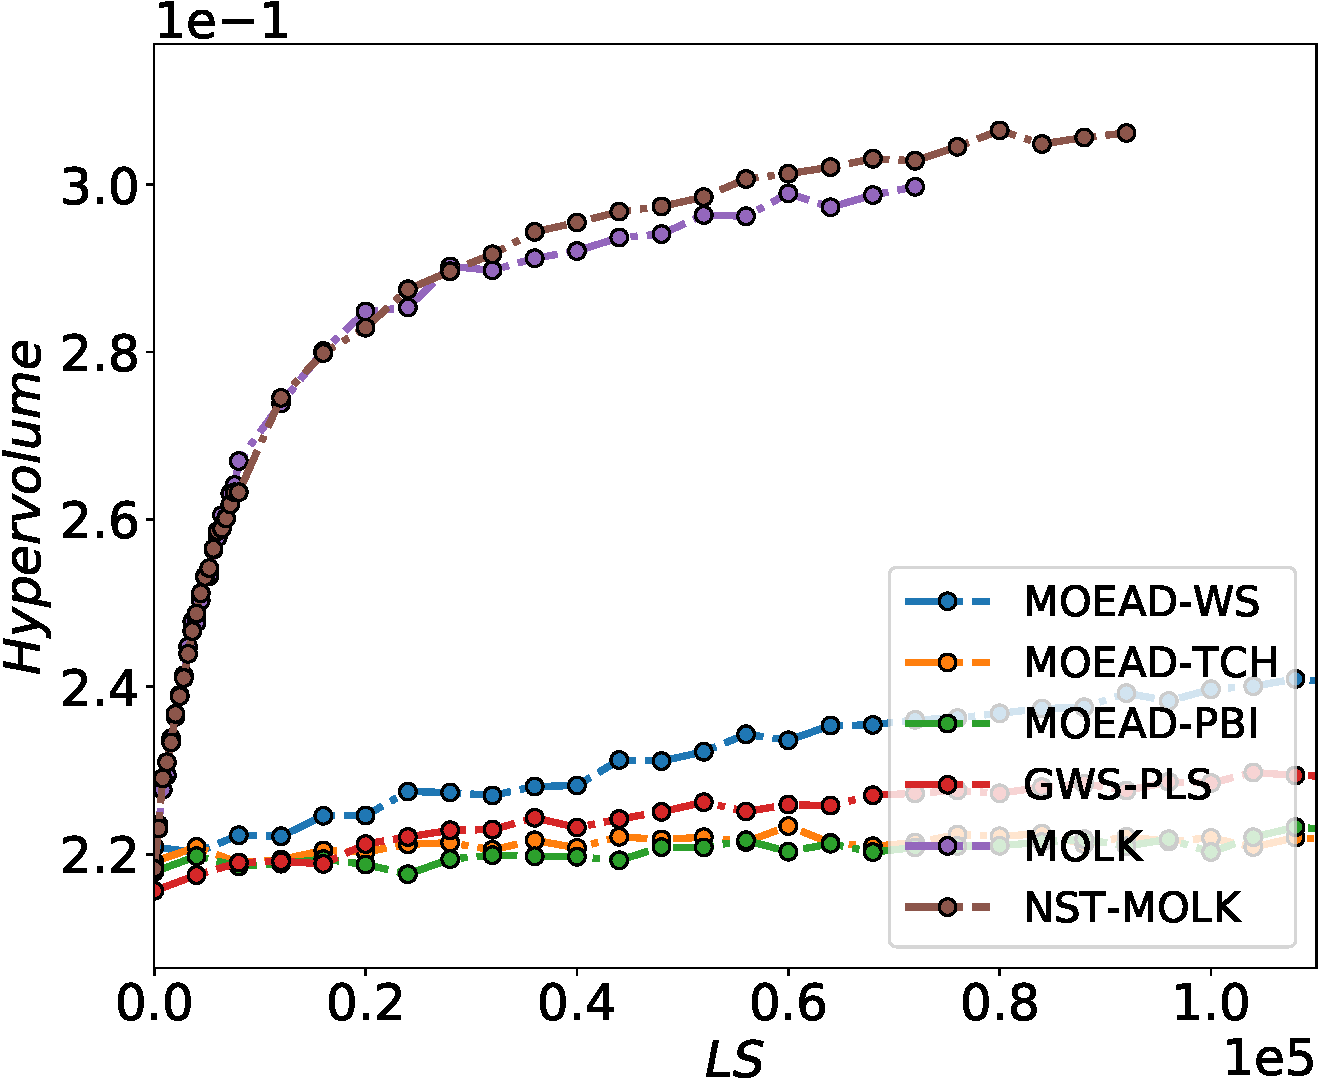
\includegraphics[width=.4\linewidth]{Convergence-LS-All-RealABCD100.pdf}
%     }
%     \caption{
%         NST-MOEA与未使用NST的NST-MOEA分别在2、3 和4目标测试用例上的收敛轨迹.
%     }
%     \label{fig:Convergence}
% \end{figure}

\subsection{两目标相似度模型有效性分析}
\label{subsec:NST:实验与讨论:两目标相似度模型有效性分析}
在本节中,将使用实验验证邻域结构迁移中的两目标相似度模型的有效性。在NST-MOEA中,两目标相似度模型的作用就在于建立起子问题和邻域结构之间的映射关系,并且为每个子问题构建一个专属的用于知识迁移的邻域结构库。为了使得算法能够尽可能的产生正迁移,子问题所属的邻域结构库中的邻域结构应该能为当前子问题带来促进的效果。如果邻域结构库中的邻域结构与当前子问题偏差很大(子问题间相似度小),那么该邻域结构所蕴含的信息就难以对当前子问题带来改进(正迁移)。若邻域结构库中的邻域结构与当前子问题没有偏差(子问题间相似度大),那么该邻域结构中所蕴含的信息就与当前子问题的邻域结构所蕴含的信息相差无几,这样就使得有很多重复的信息,也难以促进当前子问题的优化。因此,需要获取与当前子问题相似度合适的子问题下的邻域结构,而两目标相似度模型就是为了获取这样一个合适的相似度$S^*$(\autoref{eq:获取合适的相似度}),以构成邻域结构库。因此,在NST-MOEA中使用不同的相似度$S^*$对部分测试用例进行多次实验,获取平均性能最佳的相似度$S^*$,然后通过对比使用两目标相似度模型获取到的$S^*$(\autoref{tab:两目标相似度模型获取的部分相似度S*值表})是否一致,从而来验证两目标相似度模型的有效性。
\begin{table}[h]
    % \small
    % \renewcommand\tabcolsep{2pt}
    \centering
    \caption{两目标相似度模型获取的部分相似度$S^*$值表 \label{tab:两目标相似度模型获取的部分相似度S*值表}}
    \begin{tabular}{ll|ll}
        \toprule
        测试用例   & $S^*$  & 测试用例    & $S^*$ \\
        \midrule
        KroAB100          & 0.010    & EuclidAB100         & 0.010   \\
        KroAB200          & 0.011    & EuclidAB300         & 0.010   \\
        KroAB300          & 0.010    & EuclidAB500         & 0.010   \\
        KroAB400          & 0.011    & ClusterAB100        & 0.010   \\
        KroAB500          & 0.011    & ClusterAB300        & 0.010   \\
        KroAB750          & 0.010    & ClusterAB500        & 0.011   \\
        KroAB1000         & 0.011    & EuclidA$\sim$D100   & 0.019   \\
        KroABC100         & 0.005    & EuclidB$\sim$E100   & 0.019   \\
        KroBCD100         & 0.005    & EuclidA$\sim$E100   & 0.032   \\
        KroCDE100         & 0.005    & EuclidA$\sim$F100  & 0.045   \\
        KroA$\sim$D100    & 0.019    & EuclidA$\sim$G100   & 0.047   \\
        KroB$\sim$E100    & 0.019    & EuclidA$\sim$H100   & 0.047   \\
        \bottomrule
    \end{tabular}
\end{table}
\par
\begin{figure}[!h]
    \subfloat[KroAB100 \label{subfig:HV-KroAB100-Dynamic}]{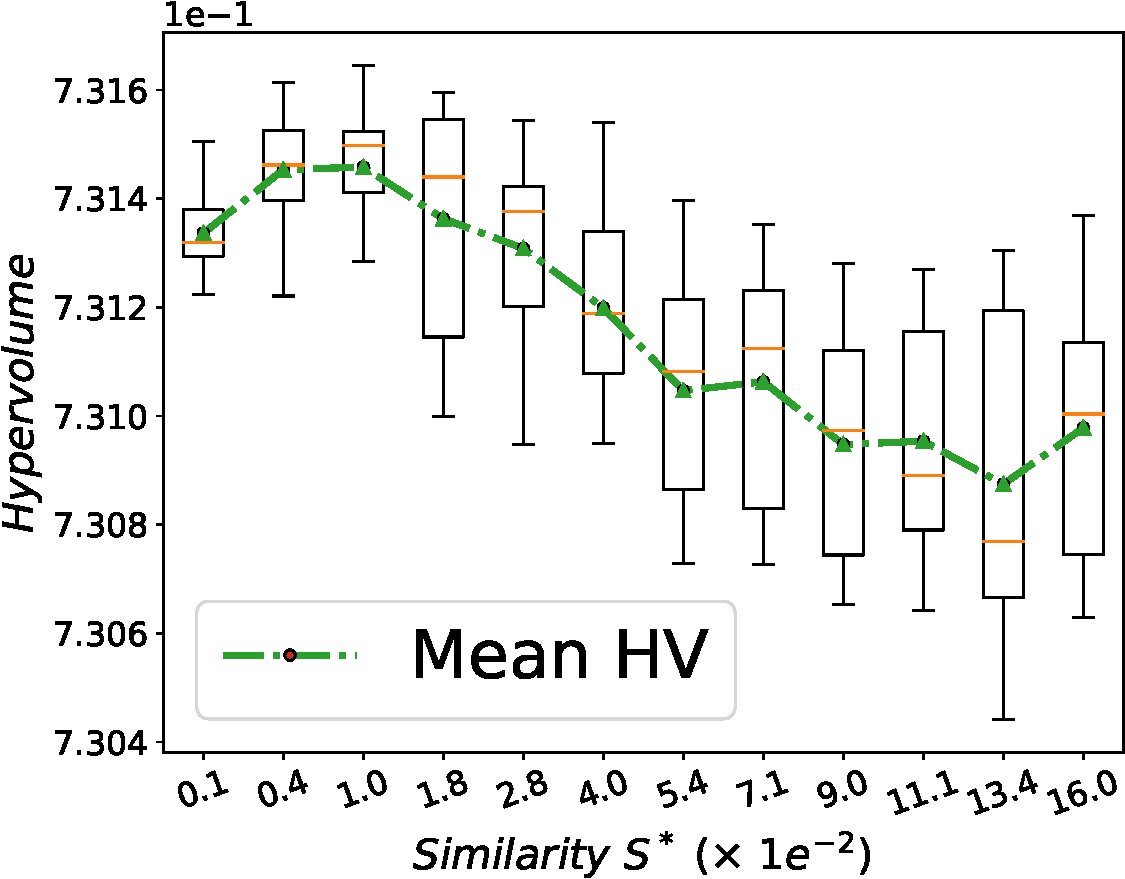
\includegraphics[width=.4\linewidth]{Similarity/Sim-HV-KroAB100-Dynamic.pdf}} \quad
    \subfloat[KroABC100 \label{subfig:HV-KroABC100-Dynamic}]{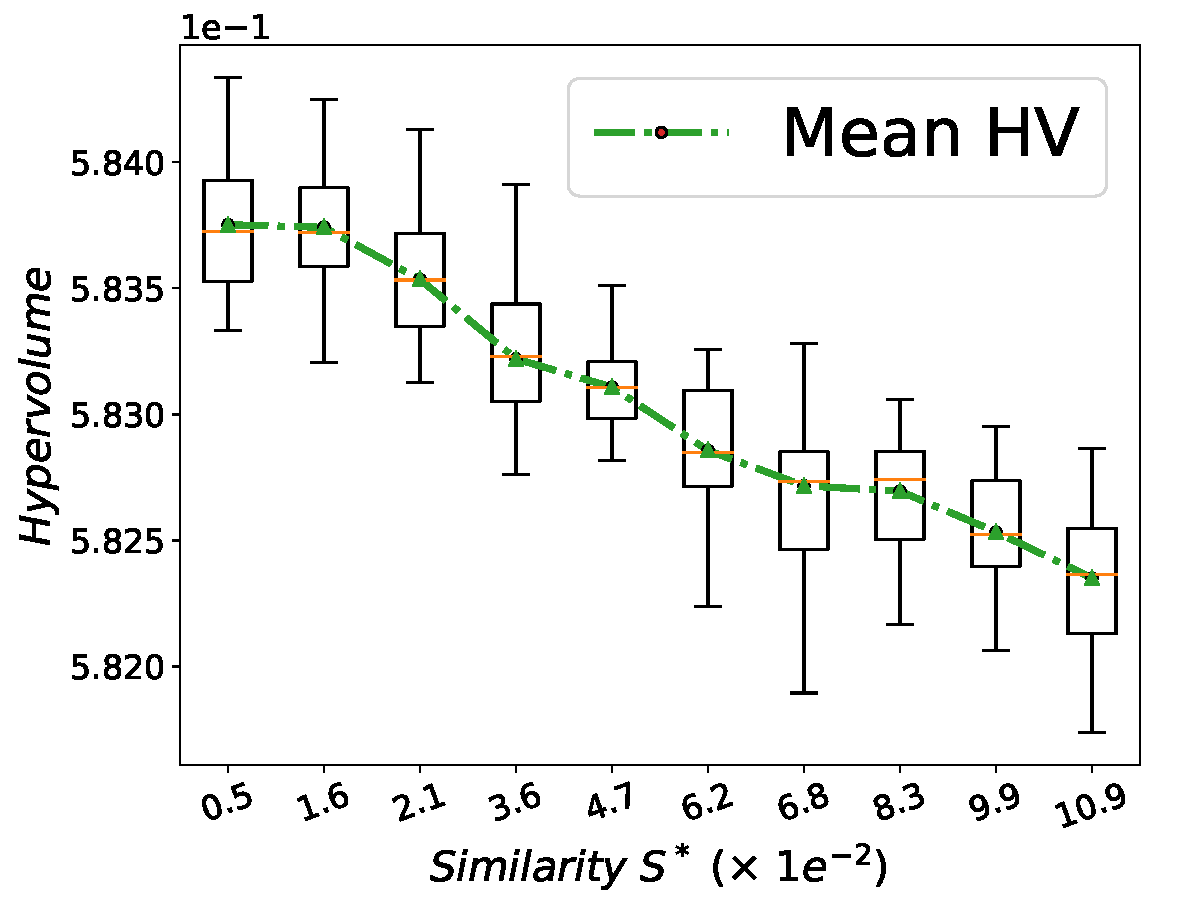
\includegraphics[width=.4\linewidth]{Similarity/Sim-HV-KroABC100-Dynamic.pdf}}\\
    \subfloat[EuclidABCD100 \label{subfig:HV-EuclidABCD100-Dynamic}]{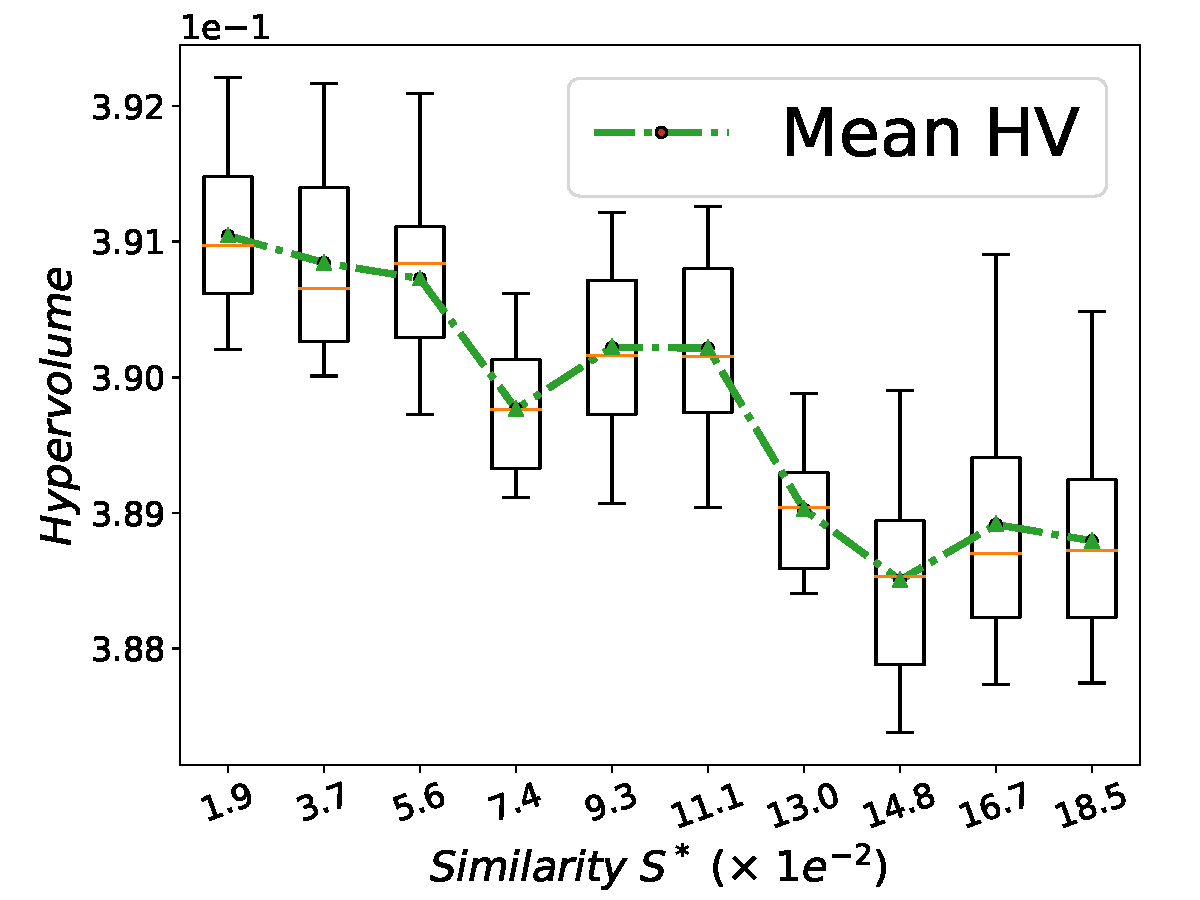
\includegraphics[width=.4\linewidth]{Similarity/Sim-HV-EuclidABCD100-Dynamic.pdf}} \quad
    \subfloat[EuclidABCDE100 \label{subfig:HV-EuclidABCDE100-Dynamic}]{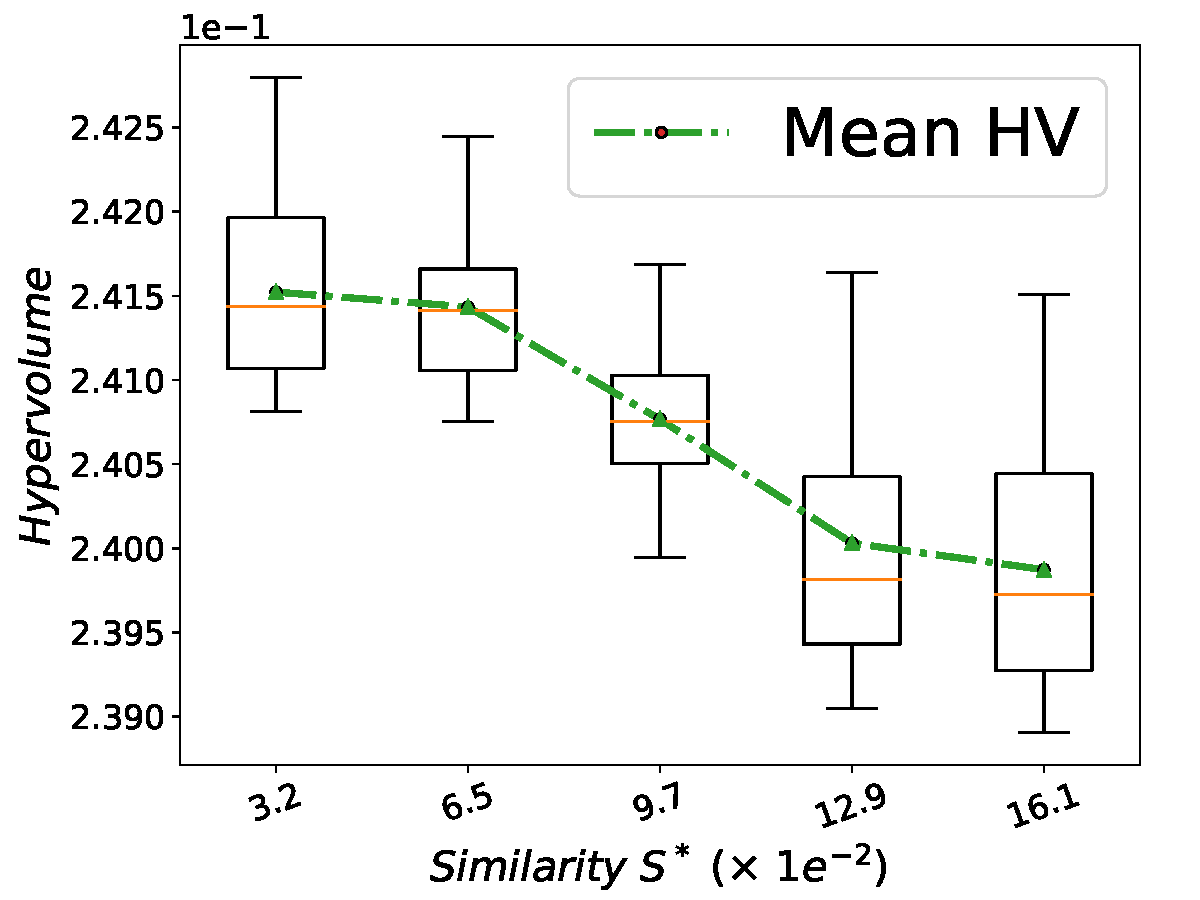
\includegraphics[width=.4\linewidth]{Similarity/Sim-HV-EuclidABCDE100-Dynamic.pdf}}
    \caption[采用不同相似度$S^*$的NST-MOEA分别在2、3、4和5目标测试用例上的Hypervolume箱型图]{采用不同相似度$S^*$的NST-MOEA分别在2、3和4目标测试用例上的Hypervolume箱型图}
    \label{fig:采用不同相似度S*的NST-MOEA分别在2、3、4和5目标测试用例上的Hypervolume箱型图}
\end{figure}
如\autoref{fig:采用不同相似度S*的NST-MOEA分别在2、3、4和5目标测试用例上的Hypervolume箱型图}~所示是采用不同相似度$S^*$的NST-MOEA分别在2、3和4目标测试用例上的Hypervolume箱型图,从图中可以观察到,当NST-MOEA的Hypervolume指标平均值最大时,此时算法表现的最好,且该指标所对应的相似度$S^*$是最优的。通过对比\autoref{fig:采用不同相似度S*的NST-MOEA分别在2、3、4和5目标测试用例上的Hypervolume箱型图}~表现最优的相似度和\autoref{tab:两目标相似度模型获取的部分相似度S*值表}~中两目标相似度模型计算得到的相似度,可以看出,两者获取的相似度在一定范围内是一致的。这说明,两目标相似度模型能够通过子问题和邻域结构之间的映射关系,找到一个合适的相似度$S^*$,从而使为子问题构建的邻域结构库中包含能够使得算法发生尽可能多的正迁移的邻域结构。由此,通过\autoref{fig:采用不同相似度S*的NST-MOEA分别在2、3、4和5目标测试用例上的Hypervolume箱型图}~和\autoref{tab:两目标相似度模型获取的部分相似度S*值表}~的对比可以证实两目标相似度的有效性。

\subsection{多臂老虎机模型有效性分析}
\label{subsec:NST:实验与讨论:多臂老虎机模型有效性分析}
在本节中,将使用实验验证邻域结构迁移中的多臂老虎机模型的有效性。在NST-MOEA中,多臂老虎机模型旨在提高算法的效率,减少计算资源。从前面的章节能够知道,在两目标相似度模型中为每个子问题都构建了邻域结构库,但是在NST-MOEA中优化子问题时,若使用该子问题邻域结构库中的所有邻域结构,这将造成大量的重复计算。并且,邻域结构库的大小和问题的目标数呈正相关,若问题的目标较多时,其邻域结构库中的邻域结构也会很多,如果每次都将邻域结构库中的所有邻域结构应用于子问题的局部搜索,则会导致算法的效率降低。由此,在NST-MOEA中使用多臂老虎机模型来为算法作出一系列的决策,从两目标相似度模型构建的邻域结构库中选出供局部搜索使用的邻域结构,使得算法的最终收益最大。为了验证多臂老虎机模型在NST-MOEA中的有效性,在子问题具有相同的邻域结构库的基础上,本节使用随机选择的方式来与使用多臂老虎机模型从邻域结构库中选择邻域结构的方式进行对比实验。
\begin{figure}[!h]
    \subfloat[KroAB100 \label{subfig:MAB-Random-Convergence-LS-KroAB100}]{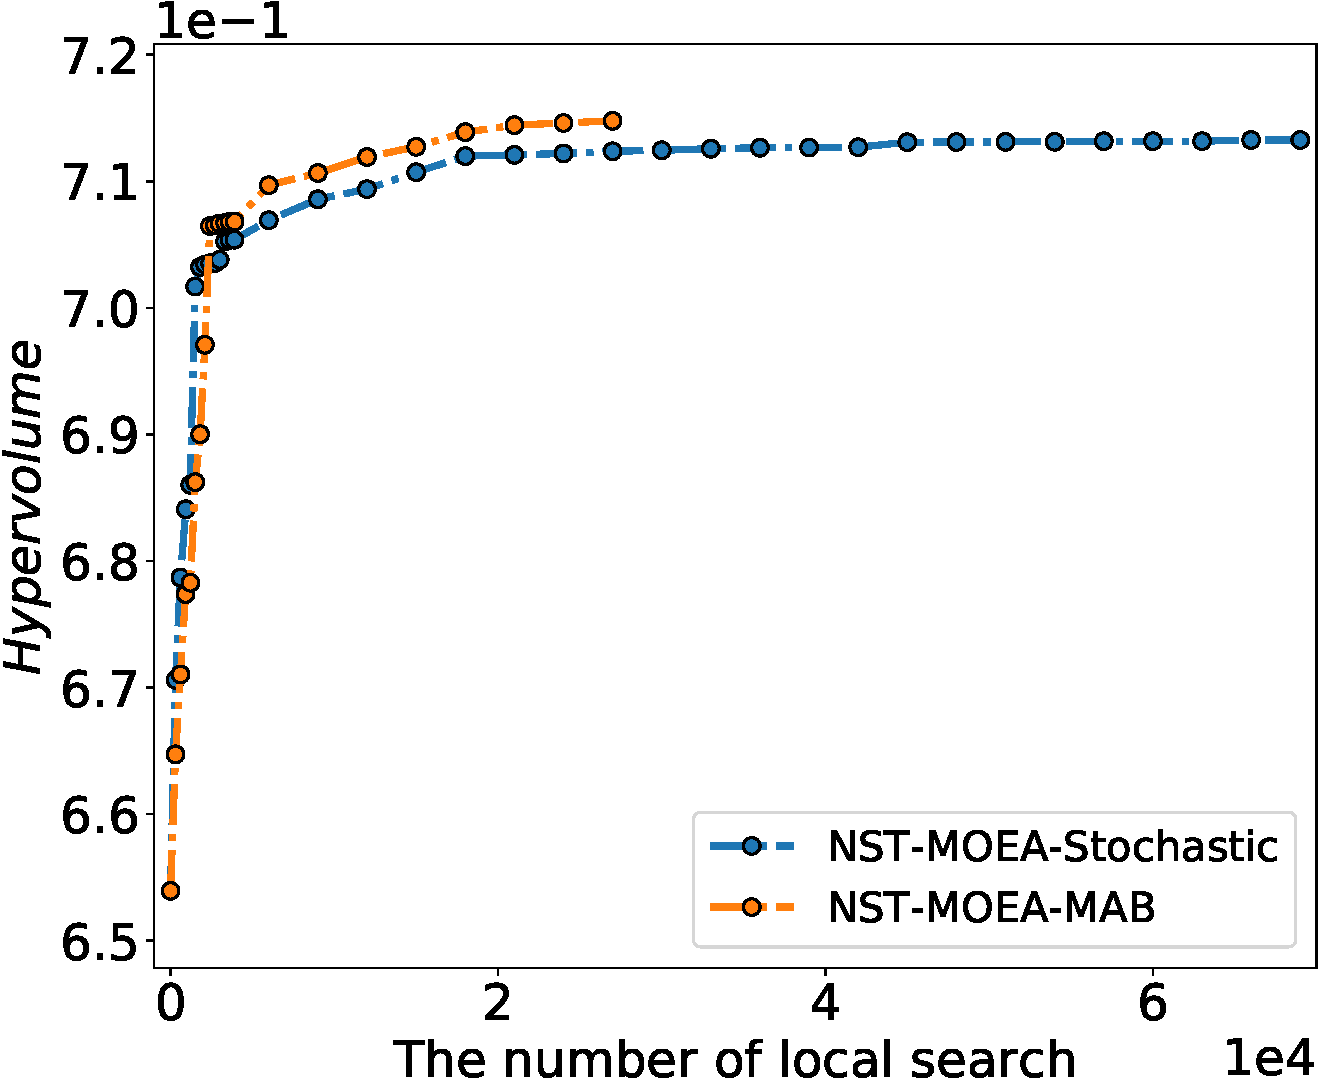
\includegraphics[width=.34\linewidth]{Ran-MAB-Convergence-LS-KroAB100.pdf}} \quad
    \subfloat[KroAB300 \label{subfig:MAB-Random-Convergence-LS-KroAB300}]{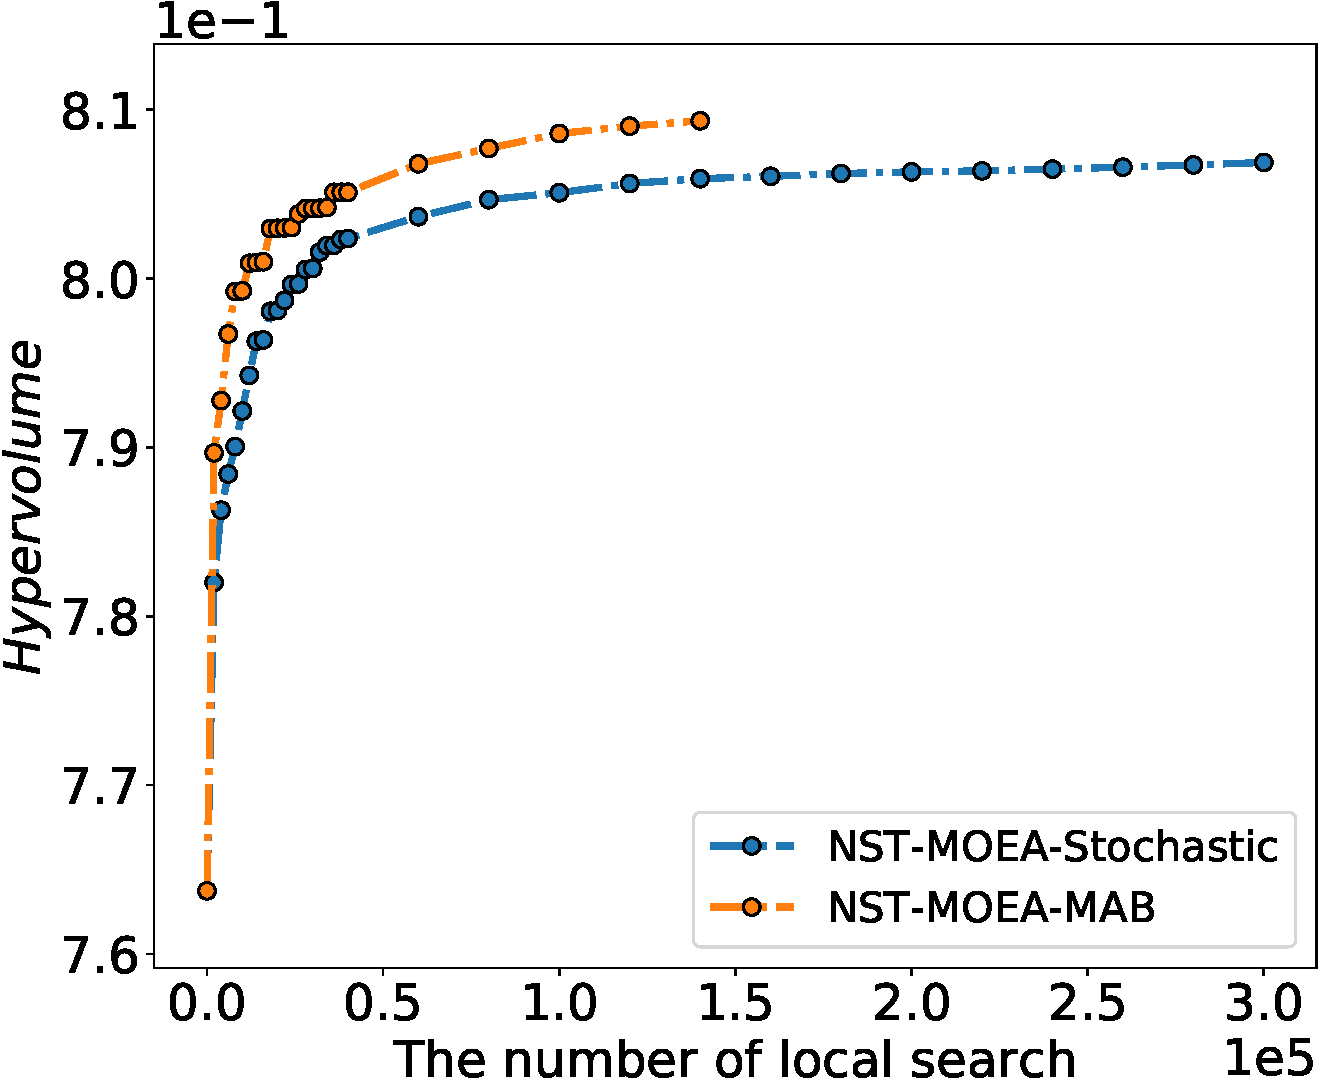
\includegraphics[width=.34\linewidth]{Ran-MAB-Convergence-LS-KroAB300.pdf}}\\
    \subfloat[KroABC100 \label{subfig:MAB-Random-Convergence-LS-KroABC100}]{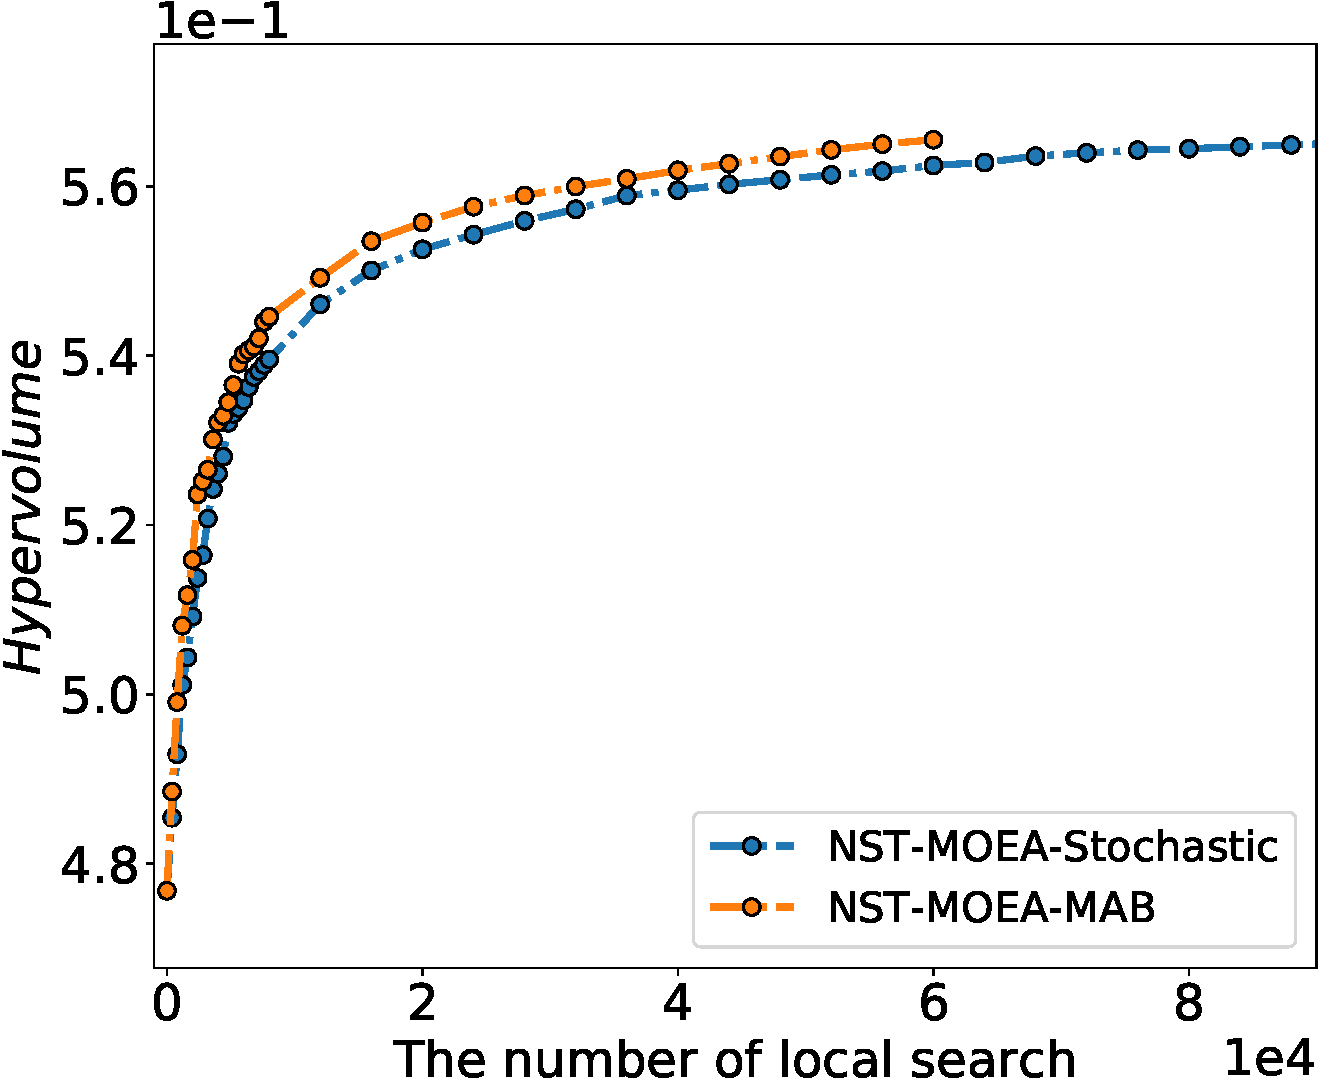
\includegraphics[width=.34\linewidth]{Ran-MAB-Convergence-LS-KroABC100.pdf}} \quad
    \subfloat[KroABCD100 \label{subfig:MAB-Random-Convergence-LS-KroABCD100}]{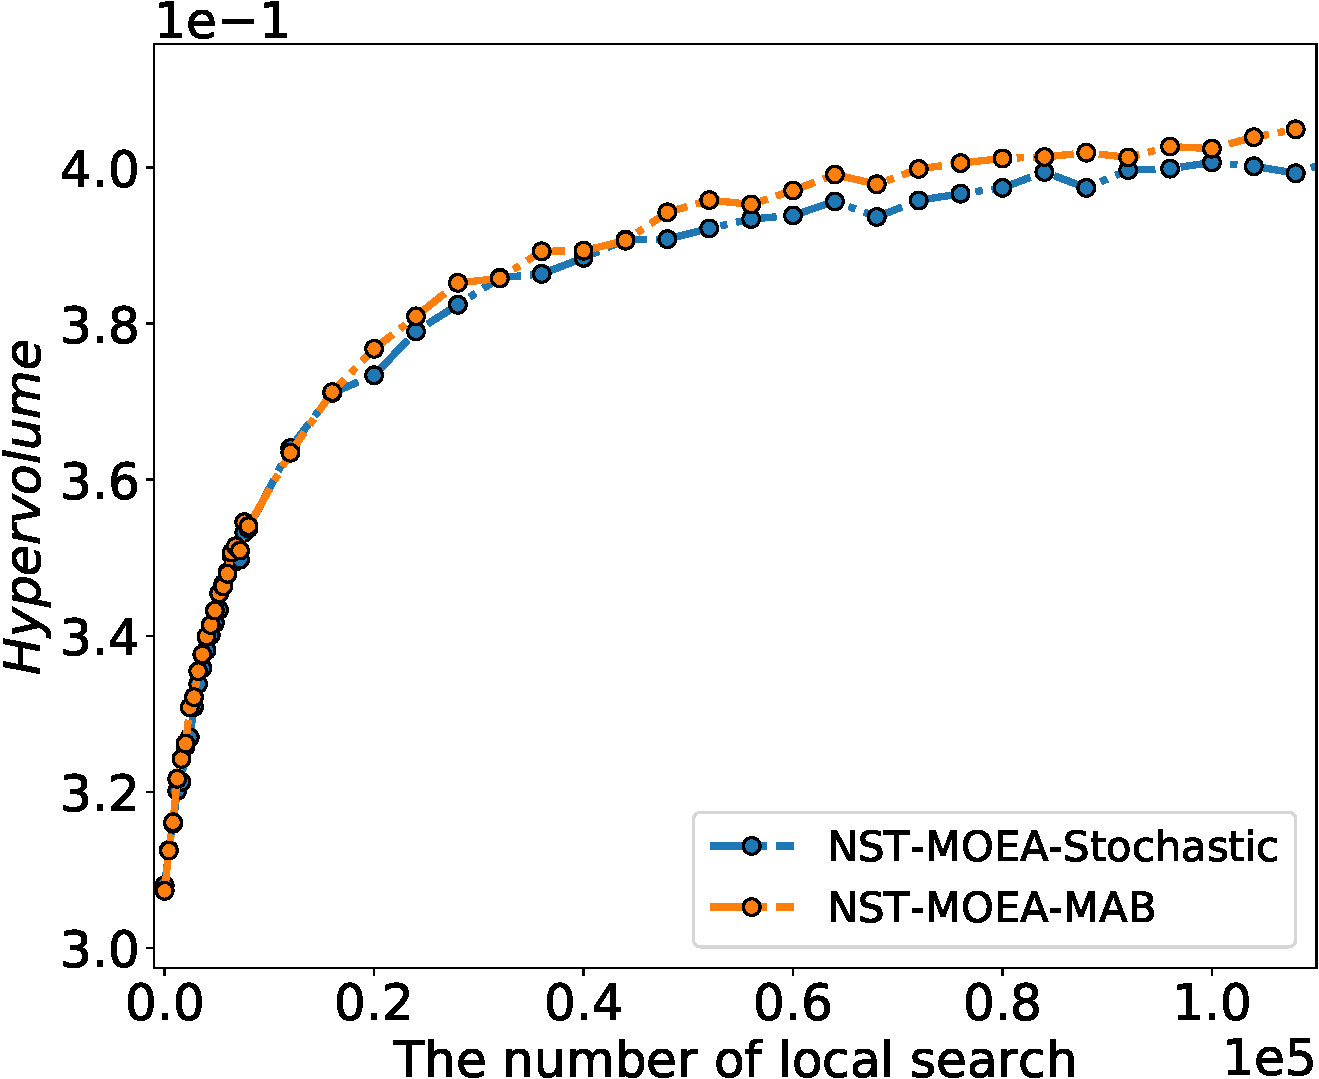
\includegraphics[width=.34\linewidth]{Ran-MAB-Convergence-LS-KroABCD100.pdf}}
    \caption[NST-MOEA中使用随机方法和MAB模型分别在2、3和4目标测试用例上的收敛轨迹]{NST-MOEA中使用随机方法和MAB模型分别在2、3和4目标测试用例上的收敛轨迹}
    \label{fig:NST-MOEA中使用随机方法和MAB模型分别在2、3和4目标测试用例上的收敛轨迹}
\end{figure}
% TODO: 改图
% \begin{figure}[!h]
%     \subfloat[KroAB100 \label{subfig:MAB-Random-HV-KroAB100}]{\includegraphics[width=.35\linewidth]{Box-HV-KroAB300.pdf}} \quad
%     \subfloat[KroAB300 \label{subfig:MAB-Random-HV-KroAB300}]{\includegraphics[width=.35\linewidth]{Box-HV-KroAB300.pdf}}\\
%     \subfloat[KroABC100 \label{subfig:MAB-Random-HV-KroABC100}]{\includegraphics[width=.35\linewidth]{Box-HV-KroAB300.pdf}} \quad
%     \subfloat[KroABCD100 \label{subfig:MAB-Random-HV-KroABCD100}]{\includegraphics[width=.35\linewidth]{Box-HV-KroAB300.pdf}}
%     \caption[NST-MOEA中使用随机方法和MAB模型分别在2、3和4目标测试用例上的Hypervolume指标箱型图]{NST-MOEA中使用随机方法和MAB模型分别在2、3和4目标测试用例上的Hypervolume指标箱型图}
%     \label{fig:NST-MOEA中使用随机方法和MAB模型分别在2、3和4目标测试用例上的Hypervolume指标箱型图}
% \end{figure}
\par
\autoref{fig:NST-MOEA中使用随机方法和MAB模型分别在2、3和4目标测试用例上的收敛轨迹}~展示的是NST-MOEA中使用随机方法和MAB模型在2、3和4目标测试用例上的收敛轨迹图,从\autoref{fig:NST-MOEA中使用随机方法和MAB模型分别在2、3和4目标测试用例上的收敛轨迹}~中能够看出,在NST-MOEA中使用MAB模型来选择邻域结构库中的邻域结构要比随机的方法收敛得要快,能够使用更少的局部搜索次数达到收敛的状态,并且目标数有多,邻域结构库中的邻域结构就越多,此时使用MAB模型的NST-MOEA的效果更加明显,以此可以验证多臂老虎机模型在NST-MOEA中的有效性。

% \autoref{fig:NST-MOEA中使用随机方法和MAB模型分别在2、3和4目标测试用例上的收敛轨迹}~和\autoref{fig:NST-MOEA中使用随机方法和MAB模型分别在2、3和4目标测试用例上的Hypervolume指标箱型图}~分别展示的是NST-MOEA中使用随机方法和MAB模型在2、3和4目标测试用例上的收敛轨迹和Hypervolume指标箱型图,从\autoref{fig:NST-MOEA中使用随机方法和MAB模型分别在2、3和4目标测试用例上的收敛轨迹}~中能够看出,在NST-MOEA中使用MAB模型来选择邻域结构库中的邻域结构要比随机的方法收敛得要快,能够使用更少的局部搜索次数达到收敛的状态,并且目标数有多,邻域结构库中的邻域结构就越多,此时使用MAB模型的NST-MOEA的效果更加明显。从\autoref{fig:NST-MOEA中使用随机方法和MAB模型分别在2、3和4目标测试用例上的Hypervolume指标箱型图}~中能够看出,使用MAB模型选择邻域结构的NST-MOEA要比使用随机方法选择邻域结构的NST-MOEA最终获得的非支配解的平均Hypervolume指标要高,这说明在NST-MOEA中使用MAB模型能够提升算法的综合性能。综上,可以验证多臂老虎机模型在NST-MOEA中的有效性。

\subsection{各算法在真实地理数据测试集上的对比}
\label{subsec:NST:实验与讨论:各算法在真实地理数据测试集上的对比}
在本节中,将会对NST-MOEA与MOEA/D(WS、TCH和PBI)、DCDG、GWS-PLS和2PPLS算法在真实地理数据测试集上进行对比。\autoref{tab:各算法在真实地理数据测试集上获得的非支配解集的Hypervolume指标对比}~和\autoref{tab:各算法在真实地理数据测试集上获得的非支配解集的C-Metric指标对比}~分别展现的是各算法在测试用例上获得的非支配解集的Hypervolume和C-Metric指标数据,从\autoref{tab:各算法在真实地理数据测试集上获得的非支配解集的Hypervolume指标对比}~和\autoref{tab:各算法在真实地理数据测试集上获得的非支配解集的C-Metric指标对比}~中能够分析出,NST-MOEA获得的非支配解集的质量在真实地理数据的测试集上的综合性能(分布性和收敛性)仍然要显著优于其他算法。尤其是在高维目标问题上,NST-MOEA的性能更加优异。此外,\autoref{fig:各算法在部分真实地理数据测试用例上的收敛轨迹示意图}~还展示了各算法在部分真实地理数据测试用例上的收敛轨迹示意图,从图中也能看出,从同一初始种群开始优化,NST-MOEA相较于其他算法,能够更快地收敛,并且使用更少的局部搜索次数。这是因为在NST-MOEA中使用局部搜索时,当子问题产生了一个优于当前个体的新解时就停止当前的局部搜索过程,而其他算法中在这个过程中并不停止,而是继续搜索完当前所有的邻居解,最后从邻居解中选出优秀的解进行更新,这就导致了浪费了大量的局部搜索操作。因此,这一操作也是NST-MOEA算法中使用局部搜索的创新点之一。
\par
{\small
\setlength{\tabcolsep}{4.5pt}
\renewcommand\arraystretch{.7}
\begin{longtable}[c]{lccccccc}
    \caption{各算法在真实地理数据测试集上获得的非支配解集的Hypervolume指标对比}\label{tab:各算法在真实地理数据测试集上获得的非支配解集的Hypervolume指标对比}\\
    \toprule
    \multirow{2}[4]{*}{测试用例} & \multicolumn{3}{c}{MOEA/D} & \multicolumn{1}{c}{\multirow{2}[4]{*}{DCDG}} & \multicolumn{1}{c}{\multirow{2}[4]{*}{GWS-PLS}} & \multicolumn{1}{c}{\multirow{2}[4]{*}{2PPLS}} & \multicolumn{1}{c}{\multirow{2}[4]{*}{NST-MOEA}} \\
    \cmidrule{2-4}          & \multicolumn{1}{c}{WS} & \multicolumn{1}{c}{THC} & \multicolumn{1}{c}{PBI} &       &       &       &  \\
    \midrule
    \endfirsthead
    \multicolumn{8}{c}{\nuaafontcaption 续表~\thetable\hskip1em 各算法在真实地理数据测试集上获得的非支配解集的Hypervolume指标对比}\\
    \toprule
    \multirow{2}[4]{*}{测试用例} & \multicolumn{3}{c}{MOEA/D} & \multicolumn{1}{c}{\multirow{2}[4]{*}{DCDG}} & \multicolumn{1}{c}{\multirow{2}[4]{*}{GWS-PLS}} & \multicolumn{1}{c}{\multirow{2}[4]{*}{2PPLS}} & \multicolumn{1}{c}{\multirow{2}[4]{*}{NST-MOEA}} \\
    \cmidrule{2-4}          & \multicolumn{1}{c}{WS} & \multicolumn{1}{c}{THC} & \multicolumn{1}{c}{PBI} &       &       &       &  \\
    \midrule
    \endhead
    \hline
    \multicolumn{8}{r}{续下页} \\
    \endfoot
    \endlastfoot
    %2 obj
    RealAB100      & 6.185e-01$^{\dag}$ & 6.253e-01$^{\dag}$ & 5.983e-01$^{\dag}$ & 6.317e-01$^{\dag}$ & 6.297e-01$^{\dag}$ & 6.308e-01$^{\dag}$ & \textbf{6.344e-01} \\
     & 4.8e-03            & 5.0e-03            & 5.9e-03            & 4.6e-03            & 4.6e-03            & 4.6e-03                          & 4.6e-03            \\
    \midrule
    RealBC100      & 6.254e-01$^{\dag}$ & 6.330e-01$^{\dag}$ & 6.099e-01$^{\dag}$ & 6.398e-01$^{\dag}$ & 6.377e-01$^{\dag}$ & 6.395e-01$^{\dag}$    & \textbf{6.431e-01} \\
               & 3.6e-03            & 3.6e-03            & 5.5e-03            & 2.7e-03            & 3.4e-03            & 2.6e-03                      & 2.5e-03            \\
    \midrule
    RealCD100      & 6.175e-01$^{\dag}$ & 6.264e-01$^{\dag}$ & 5.990e-01$^{\dag}$ & 6.318e-01$^{\dag}$ & 6.299e-01$^{\dag}$ & 6.312e-01$^{\dag}$ & \textbf{6.350e-01} \\
               & 7.0e-03            & 5.8e-03            & 6.0e-03            & 5.9e-03            & 6.1e-03            & 6.5e-03                      & 5.9e-03            \\
    \midrule
    RealAB300      & 7.737e-01$^{\dag}$ & 7.666e-01$^{\dag}$ & 7.389e-01$^{\dag}$ & 7.782e-01$^{\dag}$ & 7.761e-01$^{\dag}$ & 7.834e-01$^{\dag}$ & \textbf{7.884e-01} \\
               & 1.9e-03            & 2.6e-03            & 2.3e-03            & 1.8e-03            & 2.1e-03            & 1.8e-03                   & 1.7e-03            \\
    \midrule
    RealAB500      & 8.164e-01$^{\dag}$ & 8.060e-01$^{\dag}$ & 7.778e-01$^{\dag}$ & 8.105e-01$^{\dag}$ & 8.141e-01$^{\dag}$ & 8.220e-01$^{\dag}$ & \textbf{8.291e-01} \\
               & 1.6e-03            & 1.9e-03            & 2.3e-03            & 2.1e-03            & 1.7e-03            & 1.1e-03                       & 1.1e-03            \\
    \midrule
    RealAB750      & 8.401e-01$^{\dag}$ & 8.293e-01$^{\dag}$ & 7.996e-01$^{\dag}$ & 7.980e-01$^{\dag}$ & 8.317e-01$^{\dag}$ & 8.408e-01$^{\dag}$     & \textbf{8.515e-01} \\
               & 1.2e-03            & 1.7e-03            & 1.8e-03            & 3.0e-03            & 4.8e-03            & 1.0e-03                       & 1.1e-03            \\
    \midrule
    RealAB1000      & 8.589e-01$^{\dag}$ & 8.463e-01$^{\dag}$ & 8.177e-01$^{\dag}$ & 7.596e-01$^{\dag}$ & 8.557e-01$^{\dag}$ & 8.574e-01$^{\dag}$  & \textbf{8.695e-01} \\
               & 1.3e-03            & 1.8e-03            & 1.8e-03            & 2.7e-03            & 1.3e-03            & 1.3e-03                    & 1.2e-03            \\
    \midrule

    %3 obj
    RealABC100      & 4.268e-01$^{\dag}$ & 4.068e-01$^{\dag}$ & 3.901e-01$^{\dag}$ & 3.972e-01$^{\dag}$ & 3.956e-01$^{\dag}$ & N.A.         & \textbf{4.545e-01} \\
               & 4.0e-03            & 4.1e-03            & 4.4e-03            & 4.9e-03            & 5.9e-03            & N.A.                         & 3.6e-03            \\
    \midrule
    RealBCD100      & 4.548e-01$^{\dag}$ & 4.337e-01$^{\dag}$ & 4.153e-01$^{\dag}$ & 4.203e-01$^{\dag}$ & 4.179e-01$^{\dag}$ & N.A.                & \textbf{4.812e-01} \\
              & 5.3e-03            & 5.7e-03            & 6.0e-03            & 5.7e-03            & 8.1e-03            & N.A.                       & 4.8e-03            \\
    \midrule
    RealCDE100      & 4.575e-01$^{\dag}$ & 4.369e-01$^{\dag}$ & 4.201e-01$^{\dag}$ & 4.234e-01$^{\dag}$ & 4.232e-01$^{\dag}$ & N.A.                  & \textbf{4.842e-01} \\
             & 2.9e-03            & 3.2e-03            & 3.0e-03            & 4.1e-03            & 7.4e-03            & N.A.                          & 2.3e-03            \\
    \midrule
    %4 obj
    RealA$\sim$D100      & 2.774e-01$^{\dag}$ & 2.392e-01$^{\dag}$ & 2.472e-01$^{\dag}$ & N.A.               & 2.115e-01$^{\dag}$ & N.A.              & \textbf{3.124e-01} \\
           & 3.4e-03            & 3.7e-03            & 3.5e-03            & N.A.               & 9.1e-03            & N.A.                          & 3.3e-03            \\
    \midrule
    RealB$\sim$E100      & 2.896e-01$^{\dag}$ & 2.504e-01$^{\dag}$ & 2.579e-01$^{\dag}$ & N.A.               & 2.196e-01$^{\dag}$ & N.A.                 & \textbf{3.249e-01} \\
            & 3.0e-03            & 3.6e-03            & 3.3e-03            & N.A.               & 9.9e-03            & N.A.                          & 2.7e-03            \\
    \midrule
    RealC$\sim$F100      & 3.019e-01$^{\dag}$ & 2.618e-01$^{\dag}$ & 2.690e-01$^{\dag}$ & N.A.               & 2.285e-01$^{\dag}$ & N.A.                 & \textbf{3.375e-01} \\
            & 2.8e-03            & 3.3e-03            & 2.7e-03            & N.A.               & 8.0e-03            & N.A.                         & 2.9e-03            \\
    \midrule
    %5 obj
    Real$\sim$E100         & 1.613e-01$^{\dag}$ & 1.289e-01$^{\dag}$ & 1.428e-01$^{\dag}$ & N.A.               & 1.027e-01$^{\dag}$ & N.A.               & \textbf{1.945e-01} \\
             & 4.2e-03            & 4.2e-03            & 3.6e-03            & N.A.               & 6.3e-03            & N.A.                        & 4.1e-03            \\
    \midrule
    RealB$\sim$F100       & 1.678e-01$^{\dag}$ & 1.350e-01$^{\dag}$ & 1.496e-01$^{\dag}$ & N.A.               & 1.101e-01$^{\dag}$ & N.A.                & \textbf{2.023e-01} \\
            & 2.9e-03            & 3.6e-03            & 2.6e-03            & N.A.               & 4.7e-03            & N.A.                         & 2.9e-03            \\
    \midrule
    RealC$\sim$G100      & 1.719e-01$^{\dag}$ & 1.372e-01$^{\dag}$ & 1.530e-01$^{\dag}$ & N.A.               & 1.126e-01$^{\dag}$ & N.A.                 & \textbf{2.071e-01} \\
             & 3.1e-03            & 3.3e-03            & 2.8e-03            & N.A.               & 4.2e-03            & N.A.                        & 3.3e-03            \\
    \midrule
    %6 obj
    RealA$\sim$F100      & 8.410e-02$^{\dag}$ & 6.420e-02$^{\dag}$ & 7.295e-02$^{\dag}$ & N.A.               & 4.822e-02$^{\dag}$ & N.A.                  & \textbf{1.087e-01} \\
            & 2.1e-03            & 2.3e-03            & 1.5e-03            & N.A.               & 2.6e-03            & N.A.                         & 2.2e-03            \\
    \midrule
    RealB$\sim$G100      & 8.467e-02$^{\dag}$ & 6.465e-02$^{\dag}$ & 7.477e-02$^{\dag}$ & N.A.               & 4.897e-02$^{\dag}$ & N.A.             & \textbf{1.107e-01} \\
            & 2.2e-03            & 2.3e-03            & 1.5e-03            & N.A.               & 2.6e-03            & N.A.                          & 2.3e-03            \\
    \midrule
    RealC$\sim$H100      & 8.583e-02$^{\dag}$ & 6.515e-02$^{\dag}$ & 7.536e-02$^{\dag}$ & N.A.               & 4.914e-02$^{\dag}$ & N.A.                 & \textbf{1.118e-01} \\
          & 1.4e-03            & 1.6e-03            & 1.1e-03            & N.A.               & 2.0e-03            & N.A.                         & 1.6e-03            \\
    \midrule

    %7 obj
    RealA$\sim$FG100      & 3.343e-02$^{\dag}$ & 2.485e-02$^{\dag}$ & 3.056e-02$^{\dag}$ & N.A.               & 1.661e-02$^{\dag}$ & N.A.                & \textbf{4.817e-02} \\
      & 9.3e-04            & 9.1e-04            & 6.9e-04            & N.A.               & 1.2e-03            & N.A.                          & 1.0e-03            \\
    \midrule
    RealB$\sim$H100      & 3.506e-02$^{\dag}$ & 2.597e-02$^{\dag}$ & 3.188e-02$^{\dag}$ & N.A.               & 1.716e-02$^{\dag}$ & N.A.                 & \textbf{4.999e-02} \\
            & 8.7e-04            & 1.1e-03            & 5.3e-04            & N.A.               & 8.4e-04            & N.A.                           & 9.8e-04            \\
    \midrule
    RealC$\sim$I100      & 3.574e-02$^{\dag}$ & 2.630e-02$^{\dag}$ & 3.240e-02$^{\dag}$ & N.A.               & 1.801e-02$^{\dag}$ & N.A.                & \textbf{5.088e-02} \\
             & 7.3e-04            & 8.5e-04            & 5.7e-04            & N.A.               & 7.6e-04            & N.A.                           & 1.0e-03            \\
    \midrule

    %8 obj
    RealA$\sim$H100     & 1.601e-02$^{\dag}$ & 1.159e-02$^{\dag}$ & 1.349e-02$^{\dag}$ & N.A.               & 4.029e-03$^{\dag}$ & N.A.               & \textbf{2.407e-02} \\
           & 5.2e-04            & 4.3e-04            & 2.7e-04            & N.A.               & 1.8e-04            & N.A.                          & 6.1e-04            \\
    \midrule
    RealB$\sim$I100     & 1.609e-02$^{\dag}$ & 1.161e-02$^{\dag}$ & 1.376e-02$^{\dag}$ & N.A.               & 3.985e-03$^{\dag}$ & N.A.                 & \textbf{2.436e-02} \\
           & 4.7e-04            & 4.6e-04            & 2.4e-04            & N.A.               & 2.2e-04            & N.A.                      & 4.8e-04            \\
    \bottomrule
    \multicolumn{8}{p{45em}}{
        对Hypervolume指标值进行显著性水平为0.05的Wilcoxon秩和检验\vspace{-.75em}\newline{}
        $^\ddag$表示该算法在此问题解集上的Hypervolume指标显著优于NST-MOEA\vspace{-.75em}\newline{}
        $^\dag$表示该算法在此问题解集上的Hypervolume指标显著劣于NST-MOEA\vspace{-.75em}\newline{}
        $^\approx$表示该算法在此问题解集上的Hypervolume指标与NST-MOEA没有明显差异\vspace{-.75em}\newline{}
        N.A.表示该算法在合理的时间内无法获取该问题的非支配解集\vspace{-.75em}\newline{}
        每一行中,上面的数据为算法运行30次获取的Hypervolume指标的均值,下面的数据为标准差
        }
\end{longtable}
}% 设置字体大小,设置块
\begin{table}[!h]
    \small
    \renewcommand\arraystretch{1.2}
    \renewcommand\tabcolsep{2pt}
    \centering
    \caption{各算法在部分真实地理数据测试集上获得的非支配解集的C-Metric指标对比 \label{tab:各算法在真实地理数据测试集上获得的非支配解集的C-Metric指标对比}}
    \begin{threeparttable}
        \begin{tabular}{lcccccccccccc}
            \toprule
            \multirow{2}[4]{*}{测试用例} & \multicolumn{2}{c}{MOEA/D-WS} & \multicolumn{2}{c}{MOEA/D-TCH} & \multicolumn{2}{c}{MOEA/D-PBI} & \multicolumn{2}{c}{DCDG} & \multicolumn{2}{c}{GWS-PLS} & \multicolumn{2}{c}{2PPLS} \\
            \cmidrule{2-13}    & C(A,B)         & C(B,A)       & C(A,B)           & C(B,A)          & C(A,B)          & C(B,A)         & C(A,B)          & C(B,A)        & C(A,B)          & C(B,A) & C(A,B)          & C(B,A) \\
            \midrule
            %2 obj
            RealAB100                     & \textbf{97.63}                & 1.74                           & \textbf{80.83}                 & 4.59                     & \textbf{86.07}              & 3.17                      & \textbf{70.57}           & 10.50  & \textbf{90.77}  & 4.63   & \textbf{83.70}  & 5.78  \\
            RealBC100                     & \textbf{96.41}                & 2.39                           & \textbf{85.46}                 & 4.77                     & \textbf{87.71}              & 3.18                      & \textbf{71.12}           & 12.33  & \textbf{89.95}  & 4.77   & \textbf{81.42}  & 8.68  \\
            RealCD100                     & \textbf{96.35}                & 4.12                           & \textbf{76.88}                 & 9.50                     & \textbf{81.51}              & 6.24                      & \textbf{69.57}           & 17.39  & \textbf{86.22}  & 10.47  & \textbf{79.04}  & 13.80  \\
            RealAB300                     & \textbf{99.24}                & 0.02                           & \textbf{98.14}                 & 0.18                     & \textbf{99.51}              & 0.04                      & \textbf{93.89}           & 0.79   & \textbf{99.92}  & 0.01   & \textbf{97.94}  & 0.39  \\
            RealAB500                     & \textbf{98.82}                & 0.02                           & \textbf{98.59}                 & 0.11                     & \textbf{99.90}              & 0.00                      & \textbf{99.13}           & 0.03   & \textbf{99.97}  & 0.00   & \textbf{99.66}  & 0.02  \\
            RealAB750                     & \textbf{98.84}                & 0.02                           & \textbf{99.16}                 & 0.04                     & \textbf{99.92}              & 0.00                      & \textbf{100.00}          & 0.00   & \textbf{99.97}  & 0.00   & \textbf{99.98}  & 0.00  \\
            RealAB1000                    & \textbf{98.84}                & 0.01                           & \textbf{99.66}                 & 0.01                     & \textbf{99.84}              & 0.00                      & \textbf{100.00}          & 0.00   & \textbf{99.98}  & 0.00   & \textbf{100.00} & 0.00  \\

            %3 obj
            RealABC100                    & \textbf{57.13}                & 14.89                          & \textbf{98.06}                 & 5.14                     & \textbf{92.58}              & 5.60                      & \textbf{83.84}           & 6.61   & \textbf{85.49}  & 5.03   & N.A.            & N.A.  \\
            RealBCD100                    & \textbf{54.87}                & 12.65                          & \textbf{98.79}                 & 4.03                     & \textbf{93.25}              & 4.65                      & \textbf{86.91}           & 5.18   & \textbf{87.61}  & 4.06   & N.A.            & N.A.  \\
            RealCDE100                    & \textbf{56.98}                & 13.80                          & \textbf{98.44}                 & 4.43                     & \textbf{91.54}              & 5.20                      & \textbf{87.14}           & 5.59   & \textbf{85.68}  & 4.44   & N.A.            & N.A.  \\
            \bottomrule
        \end{tabular}
        \begin{tablenotes}
            \item[] A 代表NST-MOEA
            \item[] B 代表其他对用的算法.
            \item[] N.A. 意味着当前算法无法在合理时间内获取问题的非支配解集.
        \end{tablenotes}
    \end{threeparttable}
\end{table}
\begin{figure}[!h]
    \subfloat[RealAB100 \label{subfig:Convergence-LS-All-RealAB100}]{\includegraphics[width=.45\linewidth]{Real/Convergence-LS-All-RealAB100.pdf}} \quad
    \subfloat[RealAB300 \label{subfig:Convergence-LS-All-RealAB300}]{\includegraphics[width=.45\linewidth]{Real/Convergence-LS-All-RealAB300.pdf}}\\
    \subfloat[RealABC100 \label{subfig:Convergence-LS-All-RealABC100}]{\includegraphics[width=.45\linewidth]{Real/Convergence-LS-All-RealABC100.pdf}} \quad
    \subfloat[RealABCD100 \label{subfig:Convergence-LS-All-RealABCD100}]{\includegraphics[width=.45\linewidth]{Real/Convergence-LS-All-RealABCD100.pdf}}
    \caption[各算法在部分真实地理数据测试用例上的收敛轨迹示意图]{各算法在部分真实地理数据测试用例上的收敛轨迹示意图}
    \label{fig:各算法在部分真实地理数据测试用例上的收敛轨迹示意图}
\end{figure}

\section{本章小结}
\label{sec:NST:本章小结}
本章提出了一种基于邻域结构迁移的多目标旅行商问题求解算法(NST-MOEA)。主要针对MOTSP问题构建邻域结构,并在基于分解的多目标优化算法中使用邻域结构迁移来提升算法的性能。在NST-MOEA中,邻域结构迁移主要包含了两个模型:两目标相似度模型和多臂老虎机模型。两目标相似度模型为每个子问题构建一个能够用于知识迁移的邻域结构库,旨在加强子问题之间的信息交流,提升信息正迁移的概率。多臂老虎机模型为每一轮迭代优化的子问题选择一个邻域结构库中的邻域结构用于局部搜索,旨在选择能为当前子问题带来促进效果的知识信息,为算法优化尽可能的带来更大的收益。经过实验分析,能够说明NST-MOEA在多种类型的测试用例上都能够获得质量、性能优异的非支配解集。同时通过对比实验分析,也能够证实邻域结构迁移中的两目标相似度模型和多臂老虎机模型的有效性。